\documentclass[authoryear,12pt]{elsarticle}

\usepackage{graphicx} % Add all your packages here

\usepackage[cp1250]{inputenc}  % or [cp1250], or [latin2], or whatever
                               % suitable for your system


\usepackage{url}
%\usepackage{floatflt}
\usepackage{wrapfig}

\journal{Information Processing \& Management}


\begin{document}

\begin{frontmatter}


\title{Fuzzy Classification of Web Reports with Mining Text with Linguistic Annotations}
%
%\author{Jan Dedek and Peter Vojtas\\
%Department of Software Engineering, Charles University\\
%Institute of Computer Science, Czech Academy of Science\\
%Prague, Czech Republic\\
%email: \{jan.dedek, peter.vojtas\}@mff.cuni.cz
%%\and
%%Peter Vojtas\\
%%Department of Software Engineering, Charles University\\
%%Institute of Computer Science, Czech Academy of Science\\
%%Prague, Czech Republic\\
%%peter.vojtas@mff.cuni.cz\\
%}

%\author{Jan D\v{e}dek, Peter Vojt\'a\v{s}, Marta Vomlelov\'a}
\author[1]{Jan D\v{e}dek}
\author[1]{Peter Vojt\'a\v{s}}
\author[2]{Marta Vomlelov\'a}

\address[1]{Department of Software Engineering, Charles University,\\
Prague, Czech Republic}
\address[2]{Department of Theoretical Computer Science and Mathematical Logic,\\
Charles University, Prague, Czech Republic}

\begin{abstract}
In this paper we present a fuzzy system which provides a fuzzy
classification of textual web reports. Our approach is based on usage
of third party linguistic analyzers, our previous work on web
information extraction and fuzzy inductive logic programming. Main
contributions are: comparison of our classifier with other
alternatives like decision trees, support vector machines, neural
networks etc, extensive evaluation experiments and an introduction of
combined evaluation measures. The main conclusion is that, even under low
precision of linguistic annotation, the classification is satisfactory.
\end{abstract}

\begin{keyword}
fuzzy \sep inductive logic programming
%% keywords here, in the form: keyword \sep keyword

%% PACS codes here, in the form: \PACS code \sep code

%% MSC codes here, in the form: \MSC code \sep code
%% or \MSC[2008] code \sep code (2000 is the default)
\end{keyword}

\end{frontmatter}


\section{Introduction}
Big amount of information on the web increases the need of automated processing. Especially textual information are hard for machine processing and understanding. Crisp methods have their limitations. In this paper we present a fuzzy system which provides a fuzzy classification of textual web reports. 

\begin{figure}[hbt!]
\centerline{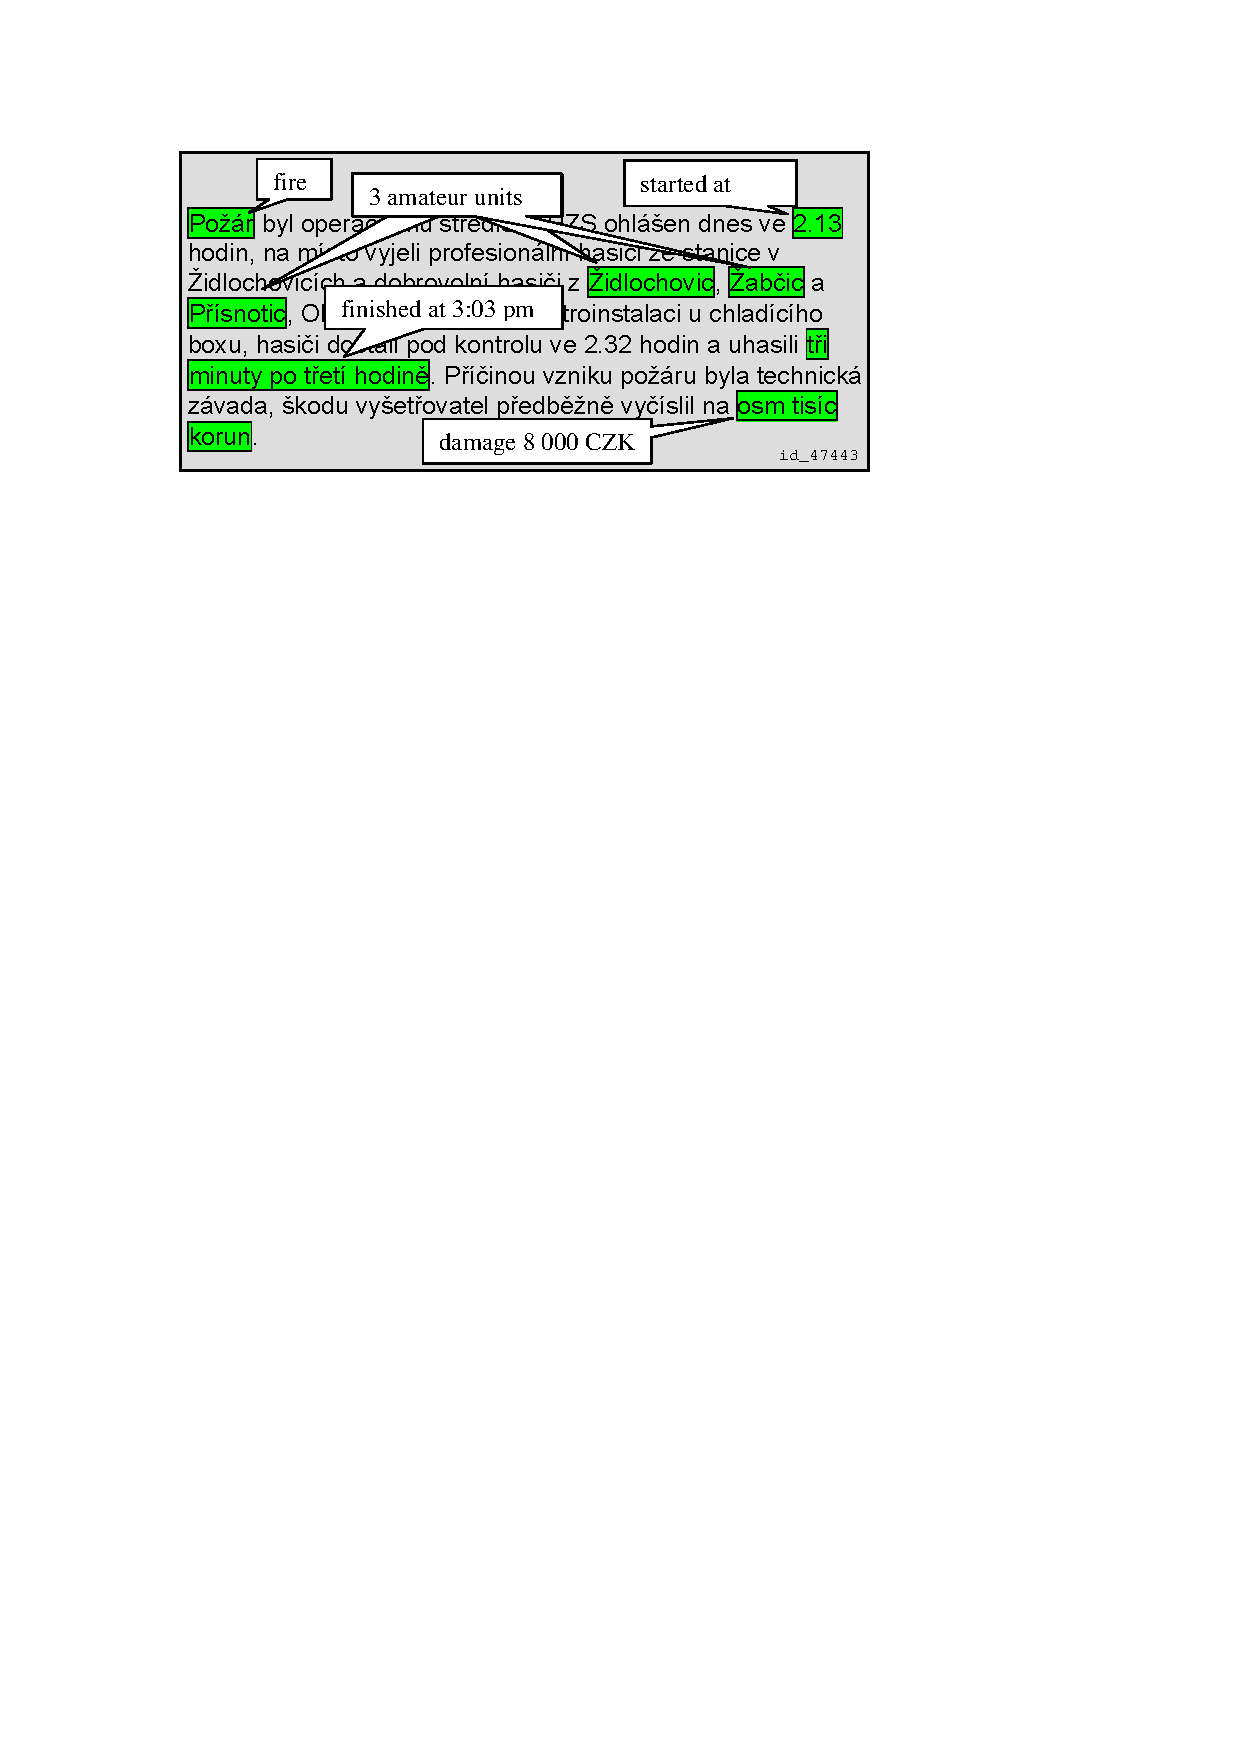
\includegraphics[width=0.7\hsize]{img/message}}
\caption{Example of analyzed web report.}
\label{dedek:message}
\end{figure}


Our motivating examples are messages of accident reports on the web (Fig.~\ref{dedek:message}). We would like to have a tool which is able to classify such message by a degree of being it a serious accident. 

Our solution is based on information extraction (see emphasized information to be extracted in the Fig.~\ref{dedek:message}) and on a machine learning procedure that gets fuzzy classification rules.




The main contributions of this paper can be stated as follows: 
\begin{itemize}
	\item formal models for fuzzy classification of information form web reports
	\item prototype implementation of a fuzzy classification system
	\item experimental evaluation of the fuzzy classification system.
\end{itemize}


\section{Related Work} \label{dedek:related}

\begin{wrapfigure}[19]{r}{.45\hsize}
\vspace{-1.5cm}
\centerline{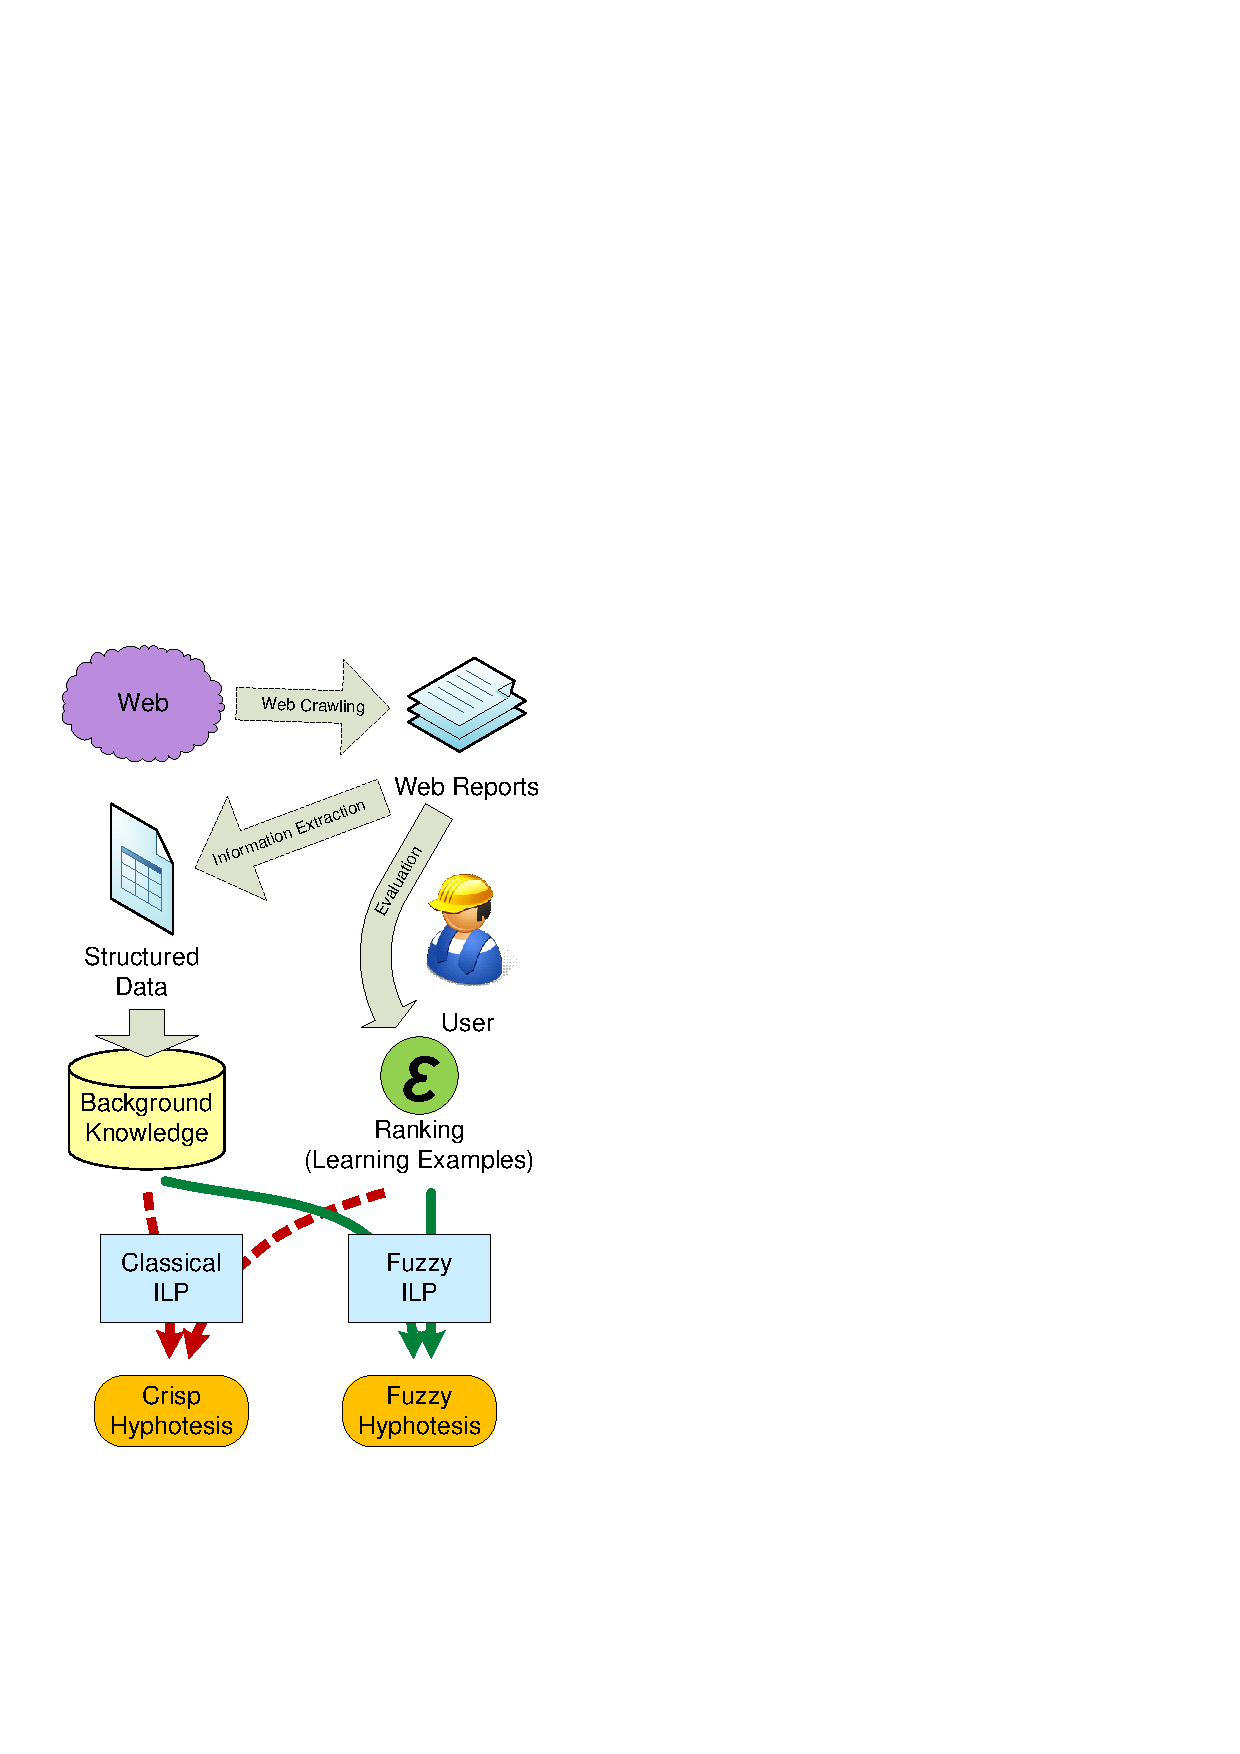
\includegraphics[width=\hsize]{img/schema}}
\caption{Schema of the whole system.}
\label{img:schema}
\end{wrapfigure}

There is a plenty of systems dealing with text mining and text classification. In \citep{dedek:ReYaLiOntoText08} the authors use ontology modeling to enhance text identification. The authors of \citep{dedek:CAP} use preprocessed data from National Automotive Sampling System and test various soft computing methods to modeling severity of injuries (some hybrid methods showed best performance). Methods of Information Retrieval (IR) are very numerous, with extraction mainly based on key word search and similarities. The Connection of IR and text mining techniques with web information retrieval can be found in Chapter Opinion mining in the book of Bing Liu \citep{dedek:WebDataMining}. 

%
%Our paper is organized as follows: In Chapter 2 we develop our models and methods and design the system, focusing on description of the linguistic analyzer, ILP, fuzzy ILP and several translations of fuzzy ILP to crisp ILP. In Chapter 3 we describe the system prototype and settings of our experiments, especially data preparation. In Chapter 4 we describe results of our experiments and provide comparison of used methods. 




%%%%%%%%%%%%%%%%%%%%%%%%%%%%%%%%%%%%%%%%%%%%%%%%%%%%%%%%%%%%%%%%%%%%%%%%%%%%%%%%%%%%%%%%%%%%%%%%%
\section{Models, methods, design of the system}
%%%%%%%%%%%%%%%%%%%%%%%%%%%%%%%%%%%%%%%%%%%%%%%%%%%%%%%%%%%%%%%%%%%%%%%%%%%%%%%%%%%%%%%%%%%%%%%%%

%\begin{floatingfigure}[r]{.45\hsize}
%\centerline{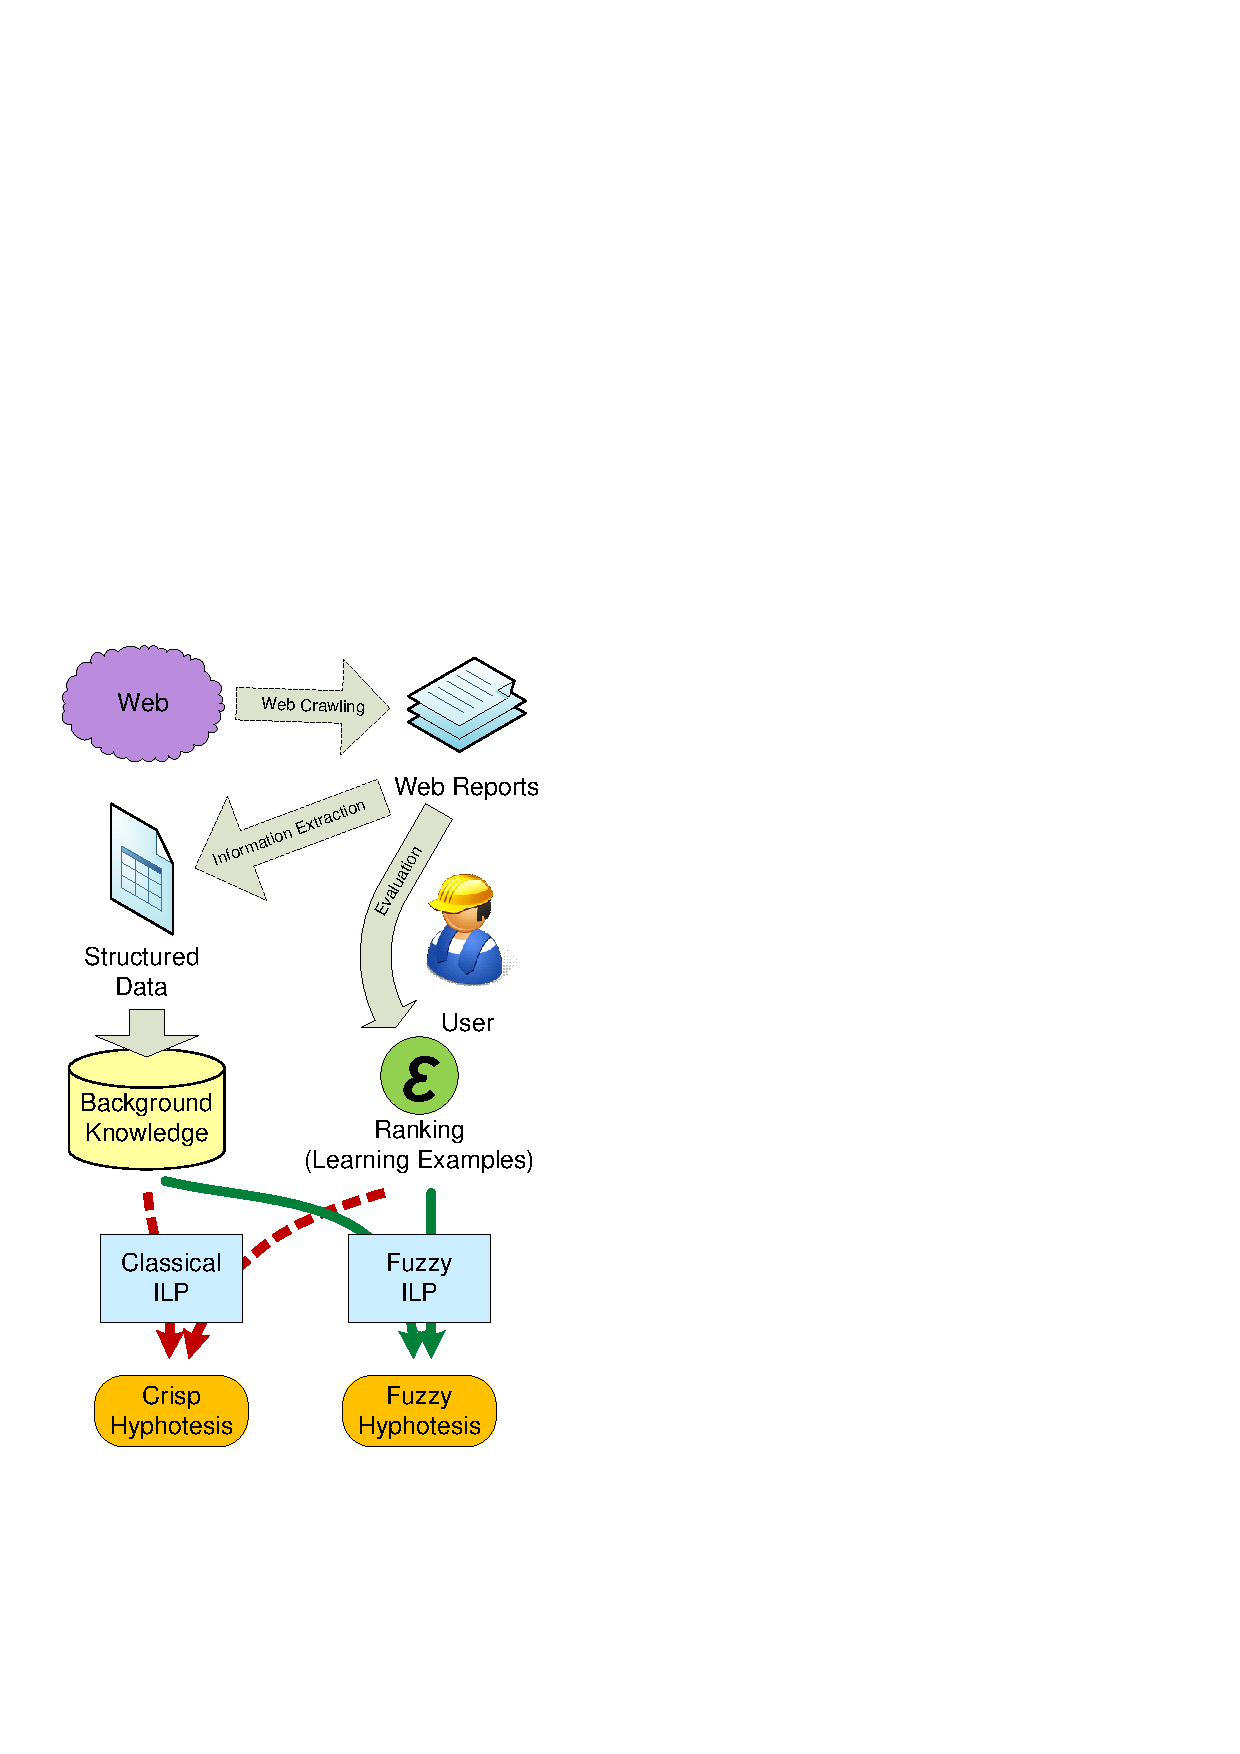
\includegraphics[width=\hsize]{img/schema}}
%\caption{Schema of the whole system.}
%\label{img:schema}
%\end{floatingfigure}

The general schema of our system is in Fig.~\ref{img:schema}. We use our previously developed web information extraction tools based on third party linguistic analyzer (the upper two dashed arrows). The classification is based on a fuzzy ILP and its translation to several crisp ILP tasks. We assume that a small amount of learning data are annotated by a human.


%\begin{figure}[hb!]
%\centerline{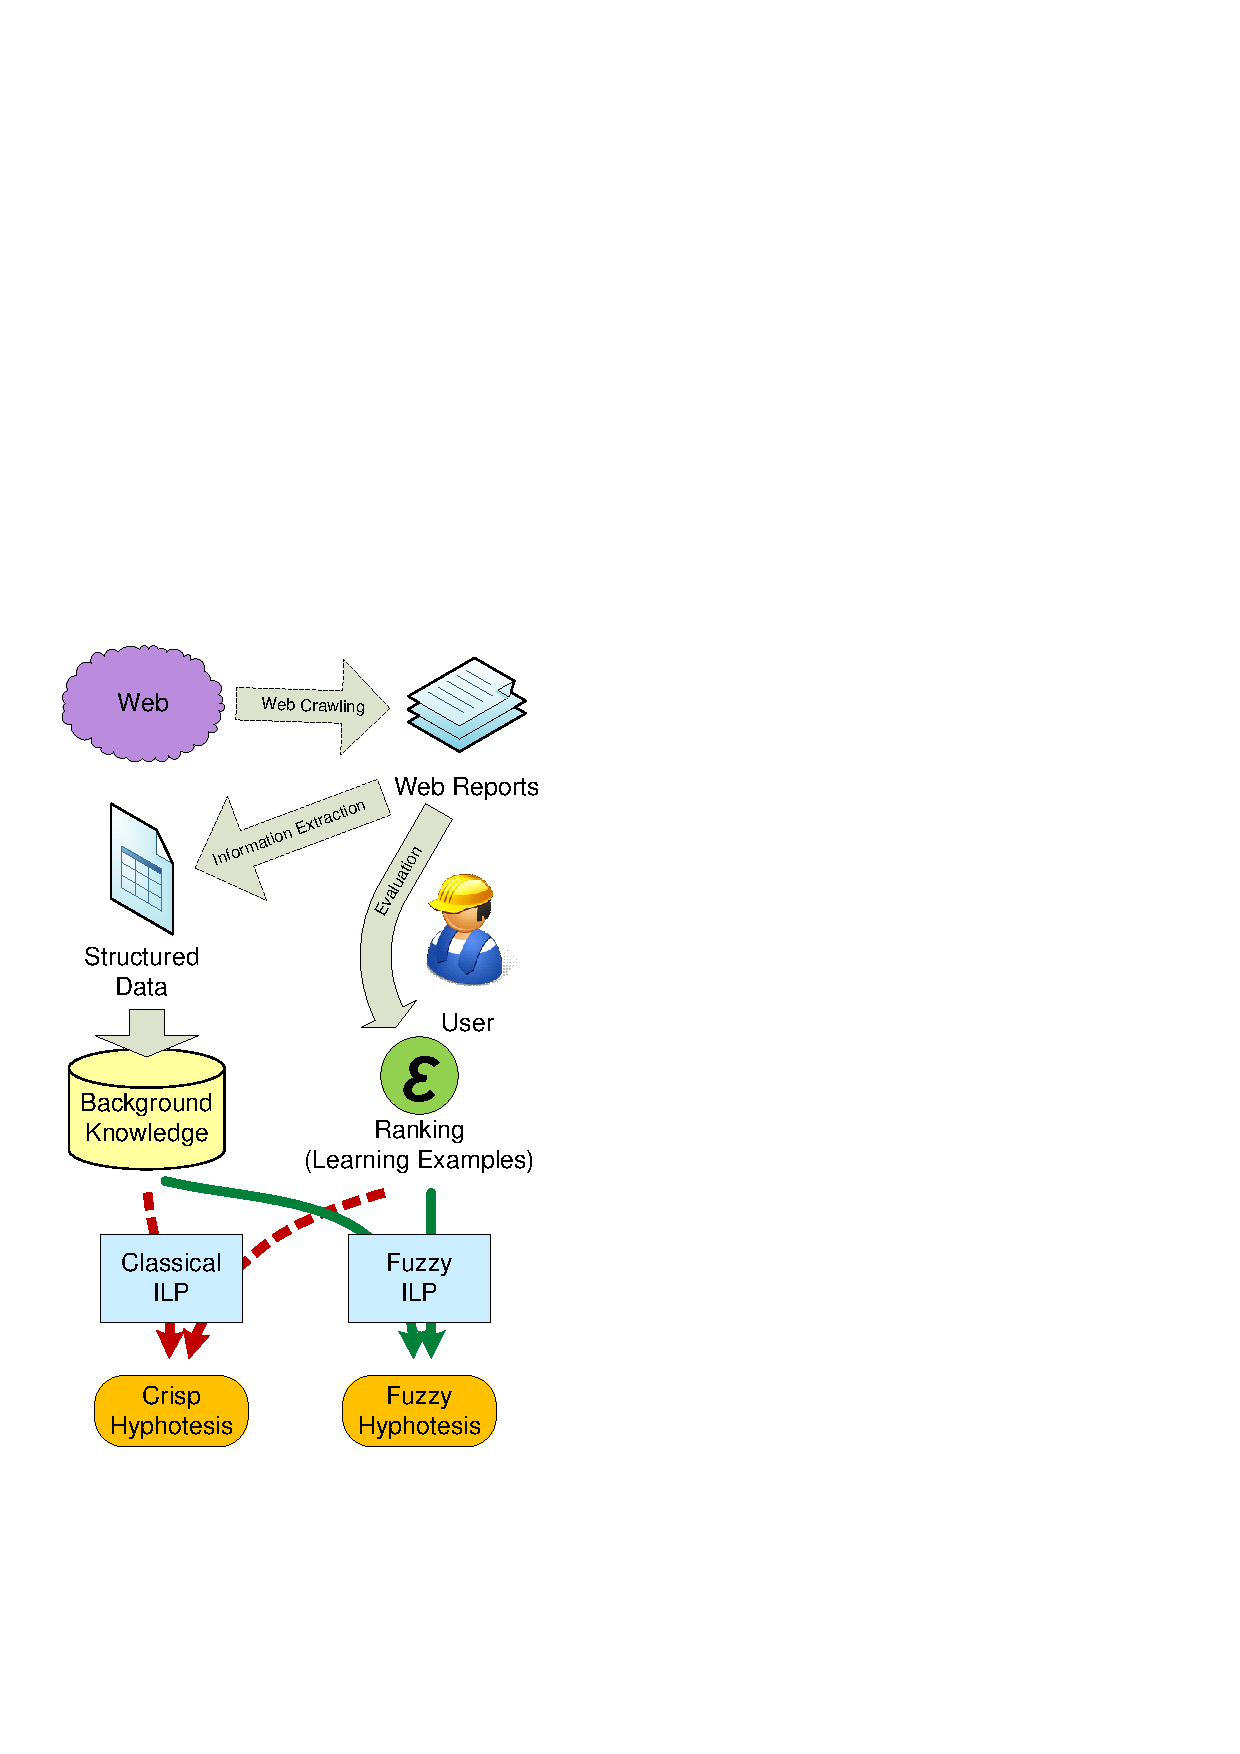
\includegraphics[width=.7\hsize,height=\hsize]{img/schema}}
%\caption{Schema of the whole system.}
%\label{img:schema}
%\end{figure}



\subsection{Linguistic Analysis}
In this section we will briefly describe the linguistic tools that
we have used to produce linguistic annotations of texts. 
These tools are being developed in the Institute of Formal
and Applied Linguistics in Prague, Czech Republic. They
are publicly available -- they have been published on a CDROM
under the title PDT 2.0 (\cite{dedek:PDT20_CD} -- first five tools) and in
(\cite{dedek:KlTransformationBasedTectogrammatical2006} -- Tectogrammatical analysis). These tools are used as a
processing chain. At the end of the chain they produce
tectogrammatical \citep{dedek:MiBeAnnotationtectogrammatical2006} dependency trees. 


\begin{description}
 
	\item[Tool 1.] Segmentation and tokenization consists of tokenization
(dividing the input text into words and punctuation)
and segmentation (dividing a sequences of tokens
into sentences).

	\item[Tool 2.] Morphological analysis assigns all possible lemmas
and morphological tags to particular word forms (word
occurrences) in the text.

	\item[Tool 3.] Morphological tagging consists in selecting a single
pair lemma-tag from all possible alternatives assigned
by the morphological analyzer.

	\item[Tool 4.] Collins' parser -- Czech adaptation. 
Unlike the usual approaches to the description of
English syntax, the Czech syntactic descriptions are
dependency-based, which means, that every edge of
a syntactic tree captures the relation of dependency
between a governor and its dependent node. Collins'
parser gives the most probable parse of a given input
sentence.

	\item[Tool 5.] Analytical function assignment assigns a description
(analytical function -- in linguistic sense) to every edge
in the syntactic (dependency) tree.

	\item[Tool 6.] Tectogrammatical analysis produces linguistic annotation
at the tectogrammatical level, sometimes called
``layer of deep syntax''. Such a tree can be seen on
the Fig.~\ref{dedek:tree}. Annotation of a sentence at this layer
is closer to meaning of the sentence than its syntactic
annotation and thus information captured at the tectogrammatical
layer is crucial for machine understanding
of a natural language \citep{dedek:KlTransformationBasedTectogrammatical2006}.
\end{description}


\subsection{Web Information Extraction}

Having web resource content analyzed by above linguistic tools, we have data stored in the form of tectogramatical trees. To achieve our objectives we have to extract information from this representation. 
Here we refer to our previous work \citep{dedek:DeVoComputingaggregations2008,dedek:DeVoLinguisticextraction2008,dedek:DeEcExperimentswith2008}. A long path of tools starting with web crawling and resulting with the extracted structured information is developed in our previous work. 
In Fig.~\ref{dedek:tree} we can see nodes of a tree where a piece of information about damage (8000 CZK) is located. We have used Inductive Logic Programming to learn rules which are able to detect such nodes. 
%In this paper we will concentrate on the usage of such extracted information to be able to classify content. 
The extraction process requires a human assistance when annotating a training data.

Note that our method is general and is not limited to Czech and can be used with any structured linguistic representation. 


\begin{figure}
\medskip
\centerline{\framebox{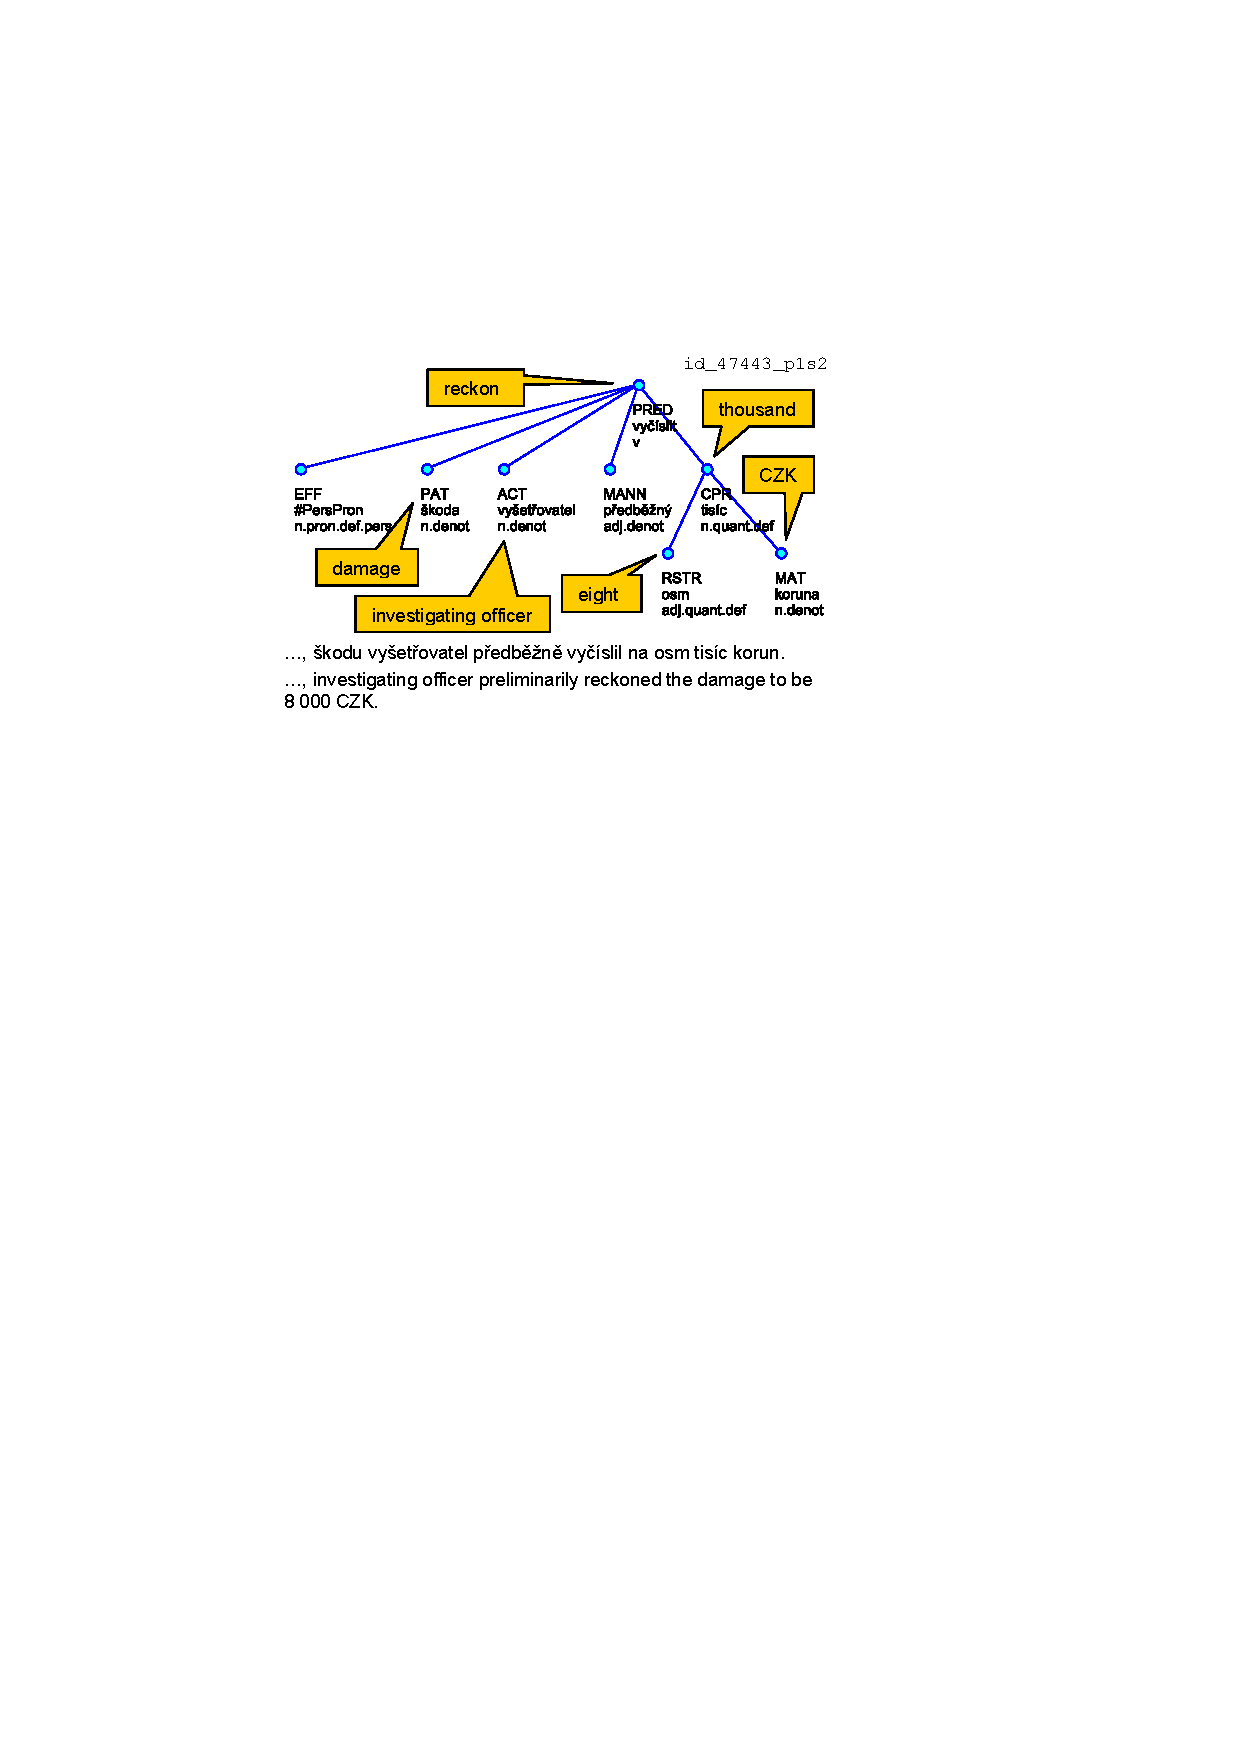
\includegraphics[width=0.7\hsize]{img/tree}}}
\caption{Example of a linguistic tree of one of analyzed sentences.}
\label{dedek:tree}
\end{figure}



\subsection{Classical ILP}

In our application we are facing the challenge of induction and/or mining on several places. First we need an inductive procedure when extracting from web texts attributes of an accident. 

Second (the subject of this paper) we need an inductive procedure when trying to explain degree of seriousness of an accident by attributes of this accident (also called background knowledge).
%
Both places where induction has to be used have following requirements


\begin{itemize}
	\item data are/can be fuzzy
	\item background knowledge is multirelational (representation of tectogramatical trees)
	\item classification is fuzzy
\end{itemize}

Having in mind these requirements we chose fuzzy inductive logic programming. To make the paper readable we present bellow short description of ILP techniques.
%

A set of examples $E=P\cup N$ is given, where $P$ contains positive and $N$ negative examples, and a background knowledge $B$. The task is to find a hypothesis $H$ such that 

$$
(\forall e\in P)(B\cup H\models e)
$$
and
$$
(\forall e\in N)(B\cup H\not\models e).
$$
Typically, $E$ consists of ground instances of the target predicate which has to be classified - in our case accidents. $B$ typically consists of several predicates (relational tables) which describe properties of object which have to be classified - in our case properties of accidents. Background knowledge can contain also some rules. Hypothesis $H$ typically consists of logic programming rules. $H$ added to $B$ entails all positive examples and no negative examples.
%
Main advantage of ILP is it's multirelational character, namely $B$ can reside in several tables.



\subsection{Fuzzy and GAP induction}

In our presentation of Inductive Logic Programming (ILP) we follow \cite{dzeroski2001:relat_dm} and  \cite{biblio:Muggleton94inductivelogic}, for fuzzy Inductive Logic Programming (fILP) we follow the paper of T. Horv\'ath and P. Vojt\'a\v s \citep{biblio:FILP} about fuzzy inductive logic programming.

We use the approach of the fuzzy logic in narrow sense developed by J. Pavelka \citep{biblio:Pavelka} and P. H\'ajek \citep{biblio:Hajek}. Formulas are of the form $\varphi, x$ ($\varphi$ is syntactically same as in the crisp case) are graded by a truth value $x\in [0,1]$.
A structure ${\mathcal M}$ consist of domain $M$ and relations are interpreted fuzzy (we do not consider function symbols here). Evaluation $\left\|\varphi\right\|_{{\mathcal M}}$ of a formula $\varphi$ uses truth functions of many valued connectives (our logic is extensional and/or truth functional). Satisfaction is defined by 
$${\mathcal M}\models_f (\varphi, x)\ iff\ \left\|\varphi\right\|_{{\mathcal M}}\ge x$$

Given is a fuzzy set of examples ${\mathcal E}:E\longrightarrow [0,1]$ and a fuzzy background knowledge ${\mathcal B}:B\longrightarrow [0,1]$. The task is to find a fuzzy hypothesis ${\mathcal H}:H\longrightarrow [0,1]$ such that 

$$(\forall e,f\in E)(\forall {\mathcal M})({\mathcal M}\models_f {\mathcal B}\cup {\mathcal H})$$
we have
$${\mathcal E}(e)>{\mathcal E}(f)\Rightarrow \left\|e\right\|_{{\mathcal M}}\ge \left\|f\right\|_{{\mathcal M}}.$$
That is, it cannot happen that
$${\mathcal E}(e)>{\mathcal E}(f) \wedge \left\|e\right\|_{{\mathcal M}}< \left\|f\right\|_{{\mathcal M}},$$
or rephrased, if ${\mathcal E}$ is rating $e$ higher than $f$, then it can not happen in a model of ${\mathcal B}\cup {\mathcal H}$ that $e$ is rated worse than $f$.

Typically, ${\mathcal E}$ consists of ground instances of the target predicate which are classified in truth degrees -- in our case degree of seriousness of an accident. ${\mathcal B}$ typically consists of several fuzzy predicates (fuzzy relational tables) which describe properties of object which have to be classified -- in our case fuzzy properties of accidents -- degree of injury, degree of damage, etc. 
%Background knowledge can contain also some rules, so far only crisp rules are used.
Hypothesis ${\mathcal H}$ typically consists of a fuzzy logic program, which when added to ${\mathcal B}$, prevents of misclassification (better can not be declared to be worse, nevertheless can be declared as having same degree (for more detailed discussion on this definition of fuzzy ILP we refer to the paper \citep{biblio:FILP})). Moreover, in practice, we use GAP -- Generalized Annotated Programs, so graded formulas will be sometimes understood as annotated (with crisp connectives and more complex annotation of head of rules). This is possible, because in \citep{biblio:KLV} we have shown that (some extension of) fuzzy logic programming is equivalent to (some restriction of) generalized annotated programs. 

\subsection{Translation of fuzzy ILP task to several classical ILP tasks}

As far as there is no implementation of fuzzy (GAP) ILP, we have to use a classical ILP system. Fortunately a fuzzy ILP task can be translated to several crisp ILP tasks (subject to some rounding and using finite set of truth values).

Assume, our fuzzy sets take values for a finite set of truth values $\{0,1\}\subseteq T\subseteq [0,1]$. For each predicate $p(x)$ in $B$ we add an additional attribute for truth value $p(x,t)$. We construct two crisp background knowledge sets  ${\mathcal B}^{raw}_T$ and ${\mathcal B}^{mon}_T$  as follows:

First is a direct coding of the fuzzy value by an additional attribute:

If ${\mathcal B}(p(x))=t\in T$, then for we add $p(x,t')\in {B}^{raw}_T$.

Second is obtained by a process called monotonization:

If ${\mathcal B}(p(x))=t\in T$, then for all $t'\in T, t'\le t$ we add $p(x,t')\in {B}^{mon}_T$.

Also example sets are constructed in two ways.

For all $t\in T$ we create a crisp example set $E_t=P_t\cup N_t$, where 
$$e\in P_t \ \ iff \ \ {\mathcal E}(e)= t$$
and $N_t$ is the rest of $E$.


For all $t\in T$ we create a crisp example set $E_{\ge t}=P_{\ge t}\cup N_{< t}$, where 
$$e\in P_{\ge t} \ \ iff \ \ {\mathcal E}(e)\ge t$$
and $N_t$ is the rest of $E$.

These two translation create two ILP tasks, first is purely crisp and second can be understood (and translated back to) fILP.

First \textit{raw ILP task} is for each $t\in T$ given by $E_t$ and $B^{raw}_{T}$, as a result we get a set of hypotheses $H_t$.

Second, for each $t\in T$ we create a crisp ILP task $E_{\ge t}, {B}^{mon}_T$ and get a hypothesis $H_{\ge t}$ guaranteeing examples of degree at least $t$. Note that variable boundings in $B$ have no boundings on truth value attribute, which was added to each predicate, and hence there are no variable boundings in $H_{\ge t}$ on truth value attribute. To predicates in $E$ we did not add the additional truth value attribute

Now we sketch the translation of second ILP task to GAP (fILP) rules. Let us assume $C$ is the target predicate in the domain of ${\mathcal E}$. We define ${\mathcal H}$ with domain consisting of one GAP rule $$C(y):u(x_1,\dots,x_m)\leftarrow B_1:x_1 \&\dots\& B_n:x_m,$$
here $B_1:x_1 \&\dots\& B_n:x_m$ is enumeration of all predicates in $B$.

Assume $B_1(y_1,t_1),\dots,B_n(y_n,t_n)$ are some predicates in $B$ (for simplicity enumerated from 1 to $n\le m$). Then for each rule 
$$R=C(y)\Leftarrow B_1(y_1,t_1),\dots,B_n(y_n,t_n)$$
in $H_t$ we give a constraint in definition of $u$ as follows
$$
U_R=u(x_1,\dots,x_m)\ge t \hbox{ if }x_1\ge t_1,\dots,x_n\ge t_n.
$$
Note that $x_{n+1},\dots,x_m$ have no restrictions.

We claim, that if all $H_t$ were correctly learned by an crisp ILP system then for $u$ the minimal solution of all constraints $U_R$ for all $R\in H_t$, for all $t\in T$, the rule
$$
C(y):u(x_1,\dots,x_m)\leftarrow B_1:x_1 \&\dots\& B_n:x_m,
$$
is a correct solution to fuzzy ILP task given by ${\mathcal E}$ and ${\mathcal B}$. Our presentation is here a little bit simplified and we freely switch between fuzzy and GAP programs, which are know to be equivalent, see  \citep{biblio:KLV}.

%%%%%%%%%%%%%%%%%%%%%%%%%%%%%%%%%%%%%%%%%%%%%%%%%%%%%%%%%%%%%%%%%%%%%%%%%%%%%%%%%%%%%%%%%%%%%%%%%
\section{The system prototype and our experiment}
%%%%%%%%%%%%%%%%%%%%%%%%%%%%%%%%%%%%%%%%%%%%%%%%%%%%%%%%%%%%%%%%%%%%%%%%%%%%%%%%%%%%%%%%%%%%%%%%%
The main experiment presented in this paper leads to the seriousness classification of an accident presented on a web report, %Our long term goal is extraction of semantic information from web reports. 
which is one of possible utilizations of the extracted information. We use web reports of fire departments of several regions of the Czech Republic. These reports are written in Czech language and can be accessed through the web of General Directorate of the Fire and Rescue Service of the Czech Republic\footnote{\url{http://www.hzscr.cz}}. 
%These reports are rich in information, e.g. where and when an traffic accident occurred, which units helped, how much time it took them to show up on the place of accident, how many people were injured, killed etc.

For our experiment we have selected a collection of 50 web reports. We have identified several features presented in these reports and manually extracted corresponding values. This will be described in more detail in section \ref{sec:features}. To each report we have also assigned a value of overall ranking of seriousness of presented accident, which is the target of the classification.

%There are two objectives to do. Fist is the web information extraction, a long path starting with web crawling and resulting with the extracted structured information. Second is the seriousness classification, which utilizes the extracted information. We have made much work on the first (see e.g. %\citep{biblio:DeVoLinguisticextraction2008,biblio:DeVoComputingaggregations2008, biblio:DeEcExperimentswith2008}), in this paper we will concentrate on the second.
%\citep{biblio:DeEcExperimentswith2008}), in this paper we will concentrate on the second.



%%%%%%%%%%%%%%%%%%%%%%%%%%%%%%%%%%%%%%%%%%%%%%%%%%%%%%%%%%%%%%%%%%%%%%%%%%%%%%%%%%%%%%%%%%%%%%%%%
\subsection{Experiment description} \label{sec:experiment_desc}
%%%%%%%%%%%%%%%%%%%%%%%%%%%%%%%%%%%%%%%%%%%%%%%%%%%%%%%%%%%%%%%%%%%%%%%%%%%%%%%%%%%%%%%%%%%%%%%%%

For the seriousness classification we have used two inductive logic approaches -- Crisp ILP and Fuzzy ILP (as described above). Technically the difference between the approaches consist in different setting of \emph{ILP task}. Both can be done with a classical ILP tool. We have used 
``\emph{A Learning Engine for Proposing Hypotheses}'' (Aleph  v5\footnote{\url{http://www.comlab.ox.ac.uk/activities/machinelearning/Aleph/}}), which seems very practical to us. It uses quite effective method of \emph{inverse entailment} \citep{biblio:InverseEntailment} and keeps all handy features of Prolog system (supports YAP and SWI) in its background.

We have compared results of the Crisp and Fuzzy ILP approaches with other classification methods and we could see that the fuzzy approach made better results than the crisp one and also than many other methods. See section \ref{sec:results} for details of the results.



\begin{table}
\centerline{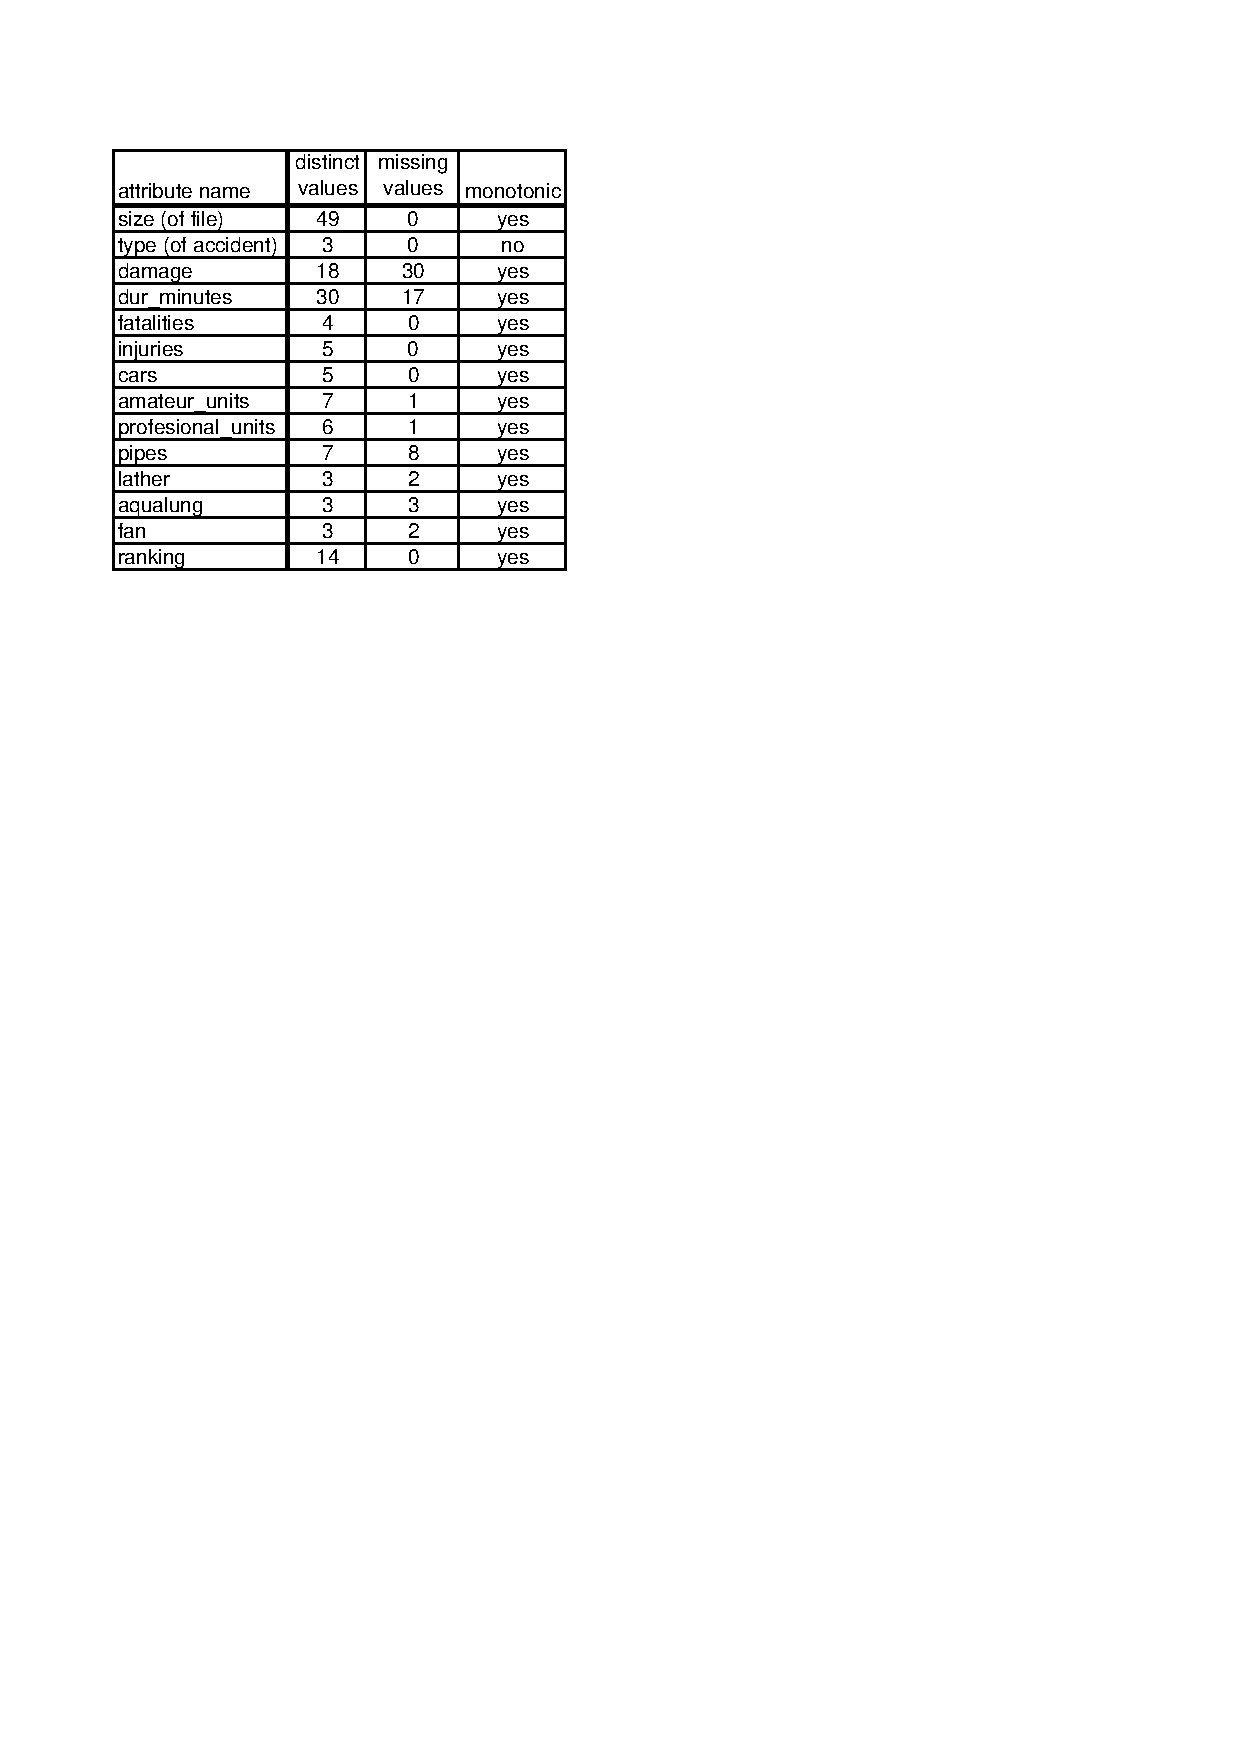
\includegraphics[width=.5\hsize]{img/attributes_description}}
\caption{Accident attributes.}
\label{img:attributes_description}
\end{table}


%%%%%%%%%%%%%%%%%%%%%%%%%%%%%%%%%%%%%%%%%%%%%%%%%%%%%%%%%%%%%%%%%%%%%%%%%%%%%%%%%%%%%%%%%%%%%%%%%
\subsection{Features of accidents} \label{sec:features}
%%%%%%%%%%%%%%%%%%%%%%%%%%%%%%%%%%%%%%%%%%%%%%%%%%%%%%%%%%%%%%%%%%%%%%%%%%%%%%%%%%%%%%%%%%%%%%%%%


%\begin{wraptable}{r}{.5\hsize}
%\centerline{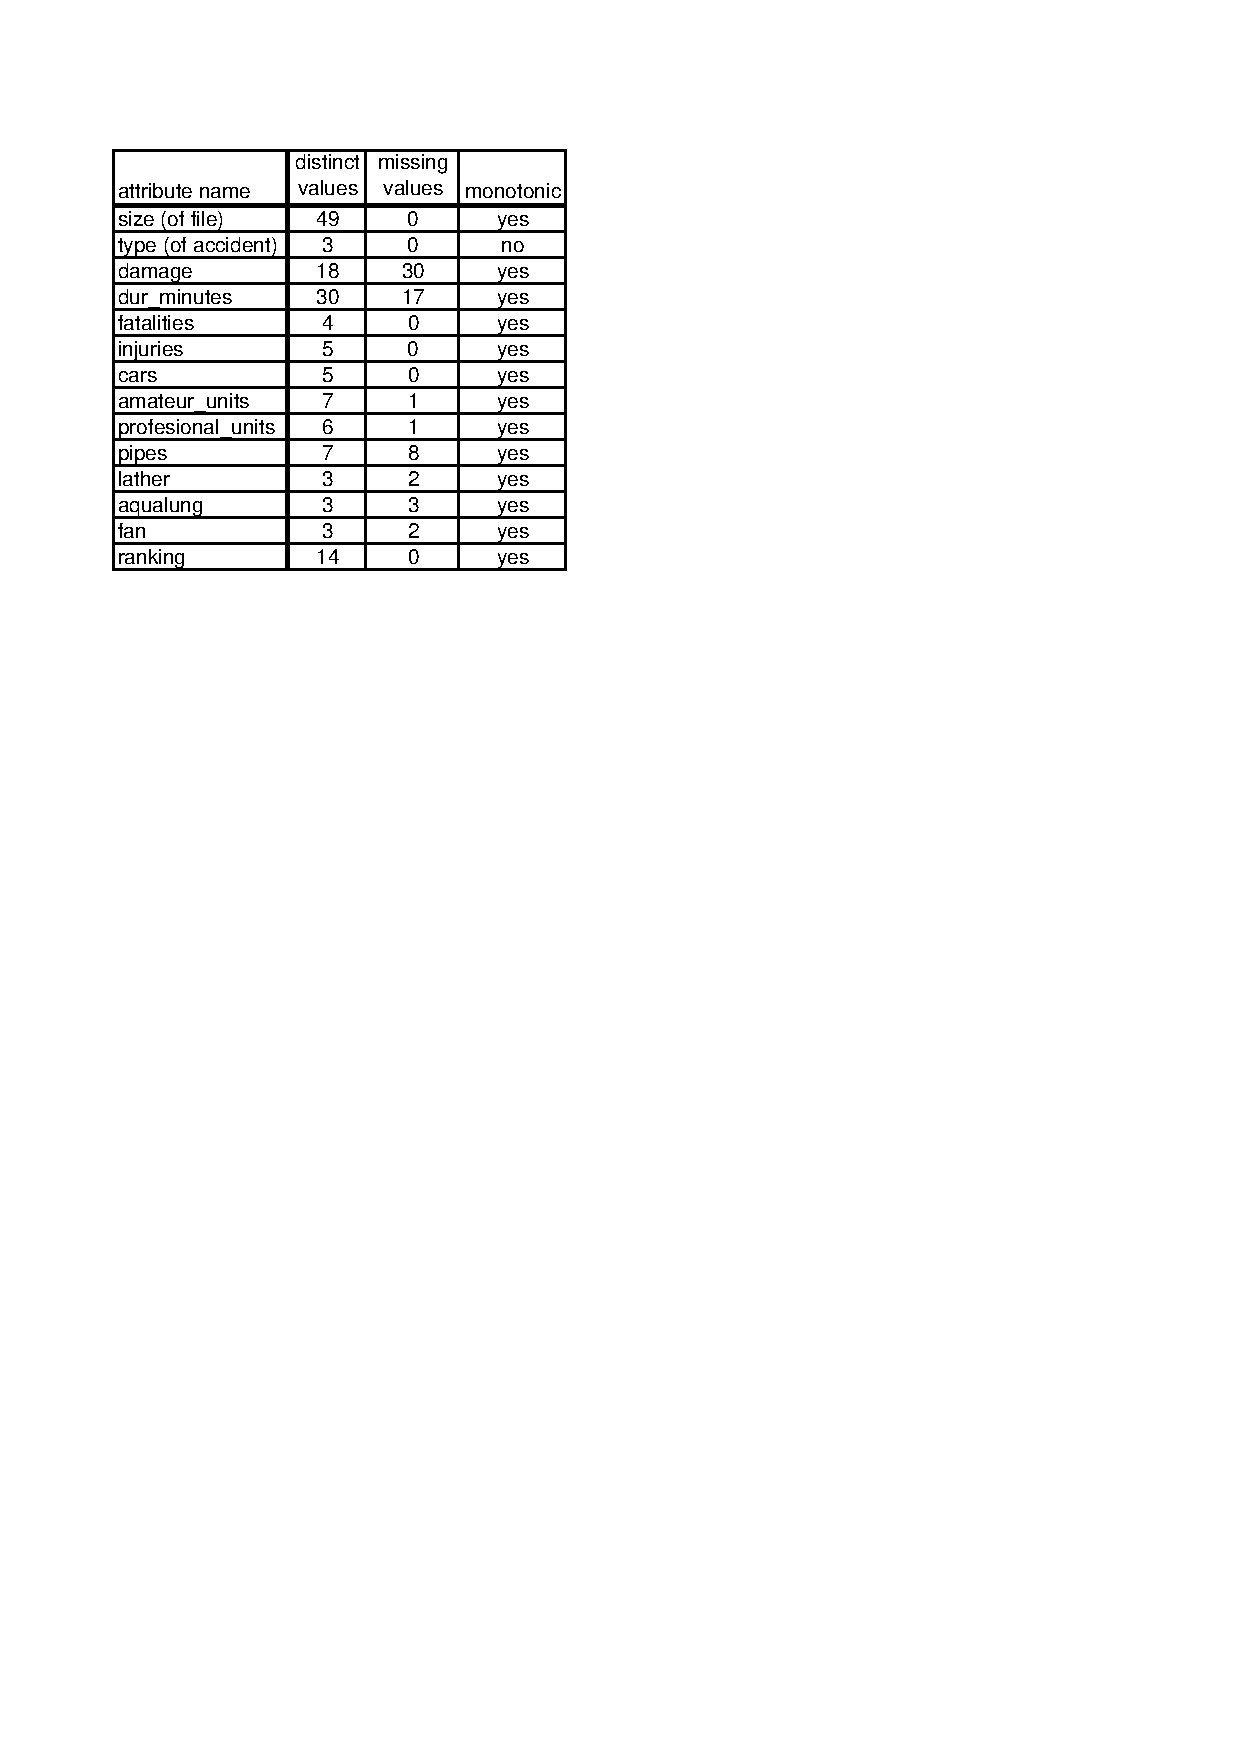
\includegraphics[width=\hsize]{img/attributes_description}}
%\caption{Accident attributes.}
%\label{img:attributes_description}
%\end{wraptable}

Table \ref{img:attributes_description} summarizes all features (or attributes) that we have obtained from accident reports. Except the attribute \verb+type+ (type of an accident -- \verb+fire+, \verb+car_accident+ and \verb+other+) all the attributes are numerical and so monotonizable. There are cases when the value of an attribute is unknown. We have decided to make evidence of this and keep the values \verb+unknown+ in our knowledge base. A brief explanation of each attribute follows.
\begin{itemize}
	\item \verb+size+ is a file size of text part of a report.
	\item \verb+damage+ is an amount (in CZK -- Czech Crowns) of summarized damage arisen during an accident.
	\item \verb+dur_minutes+ is time taken to handle an accident.
	\item \verb+fatalities+ and \verb+injuries+ are numbers of fatalities (and injuries) taken by an accident.
	\item \verb+cars+ is number of cars damaged during an accident (especially during car accidents).
	\item \verb+professional_units+ and \verb+amateur_units+ are numbers of fireman units sent for an accident.
	\item \verb+pipes+ is number of  used fire pipes.
	\item \verb+lather+, \verb+aqualung+ and \verb+fan+ (ventilator) indicates whether these devices were used.
\end{itemize}


%%%%%%%%%%%%%%%%%%%%%%%%%%%%%%%%%%%%%%%%%%%%%%%%%%%%%%%%%%%%%%%%%%%%%%%%%%%%%%%%%%%%%%%%%%%%%%%%%
\subsection{Seriousness ranking} \label{sec:seriousness}
%%%%%%%%%%%%%%%%%%%%%%%%%%%%%%%%%%%%%%%%%%%%%%%%%%%%%%%%%%%%%%%%%%%%%%%%%%%%%%%%%%%%%%%%%%%%%%%%%

%\vspace{0.2cm}
%\noindent \textbf{Seriousness ranking}

\begin{figure}
\centerline{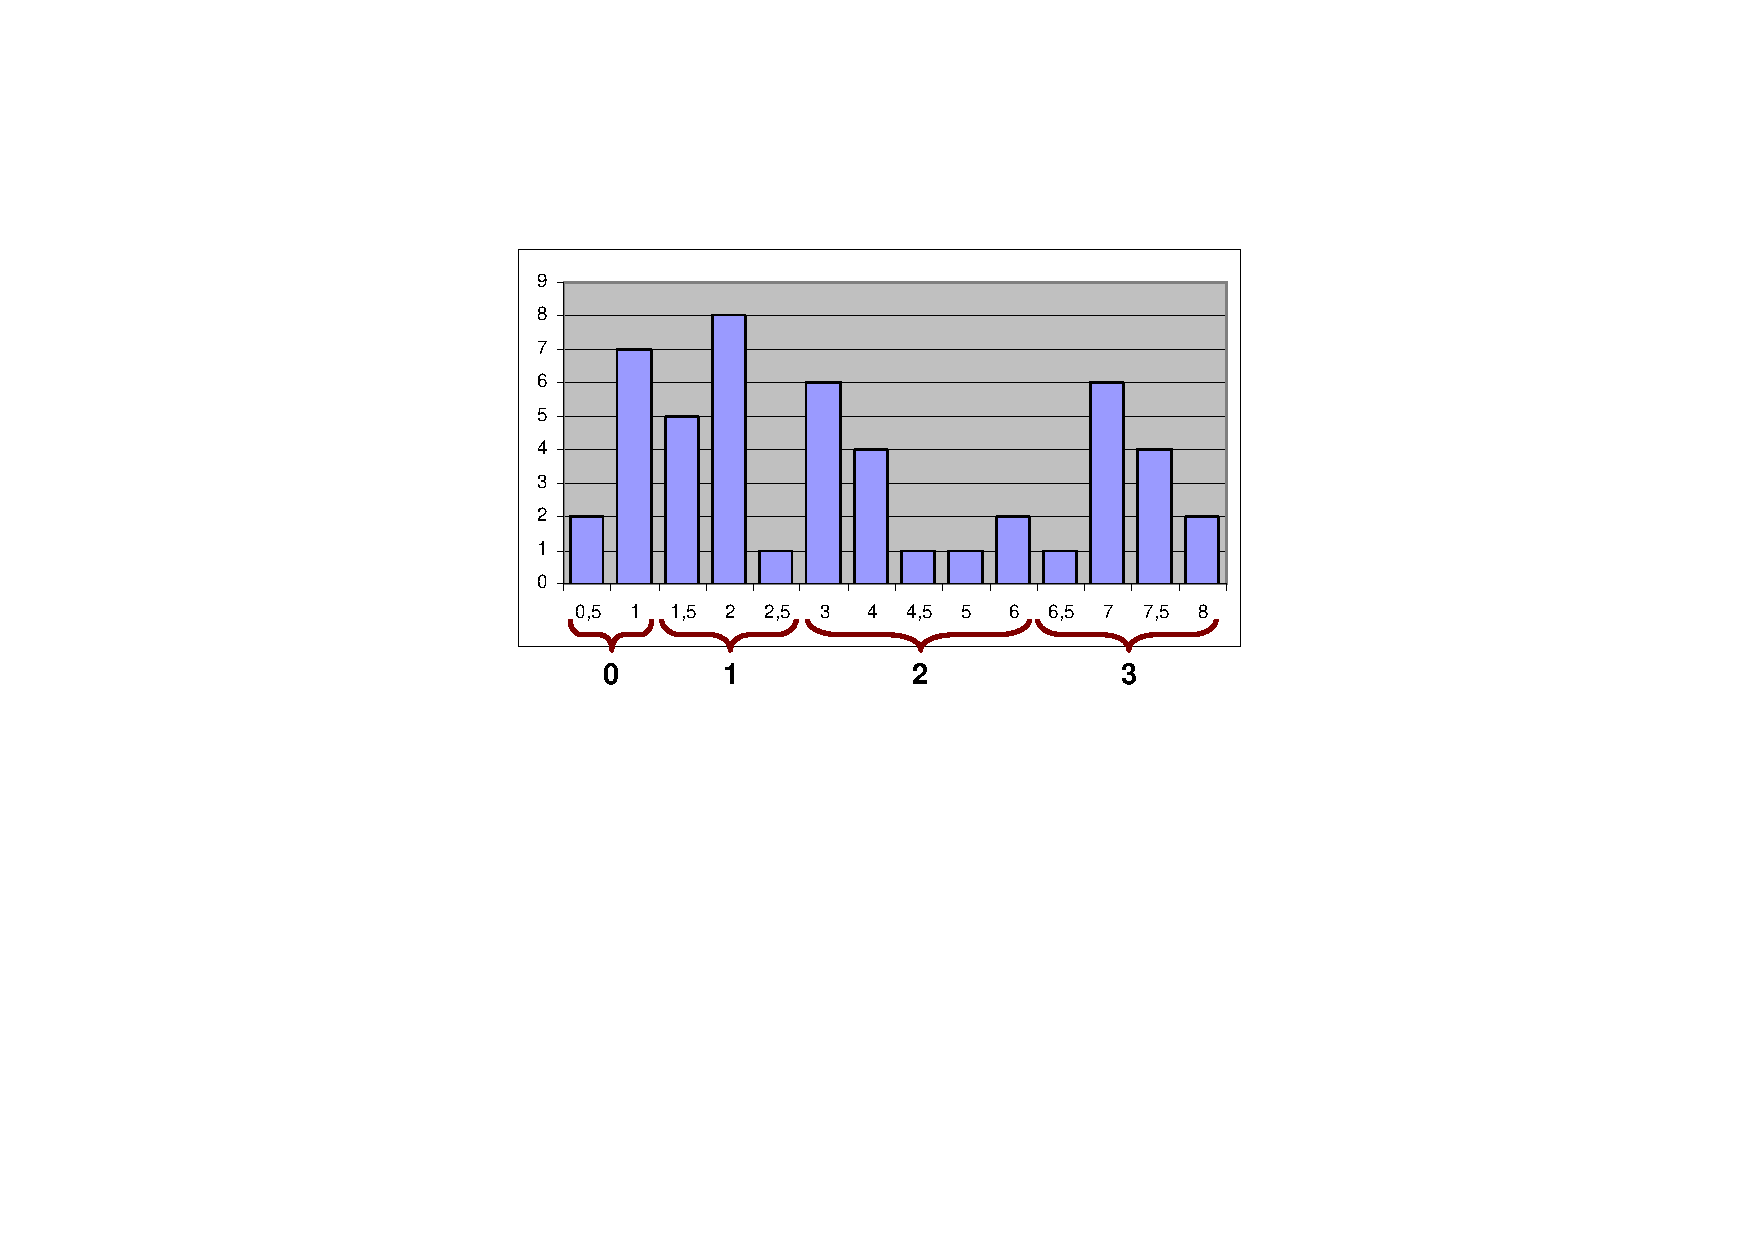
\includegraphics[width=0.7\hsize]{img/ranking_histogram}}
\caption{Frequencies of accident ranking.}
\label{img:ranking_histogram}
\end{figure}

\noindent Values of overall seriousness ranking attribute were stated from ``general impression'' from report's texts with respect to the particular attributes. %(Fig.~\ref{img:attributes_description}). 
Values of seriousness ranking have evolved to 14 distinct values in range form 0.5 to 8. 
Histogram with frequencies of all the values is on the Figure~\ref{img:ranking_histogram}.
We have divided the values into four approximately equipotent groups 
(see in the Fig.~\ref{img:ranking_histogram}) 
and these groups determine the target class attribute in our classification task. 
%and logic rules were learned for each group separately\footnote{We do not have a binary rule which would return an exact value of the rating, but we have one ``true/false'' rule for each of the four categories.}.



\begin{figure}[htb]
\begin{minipage}[b]{0.5\hsize}
	Crisp learning examples\\
	\centerline{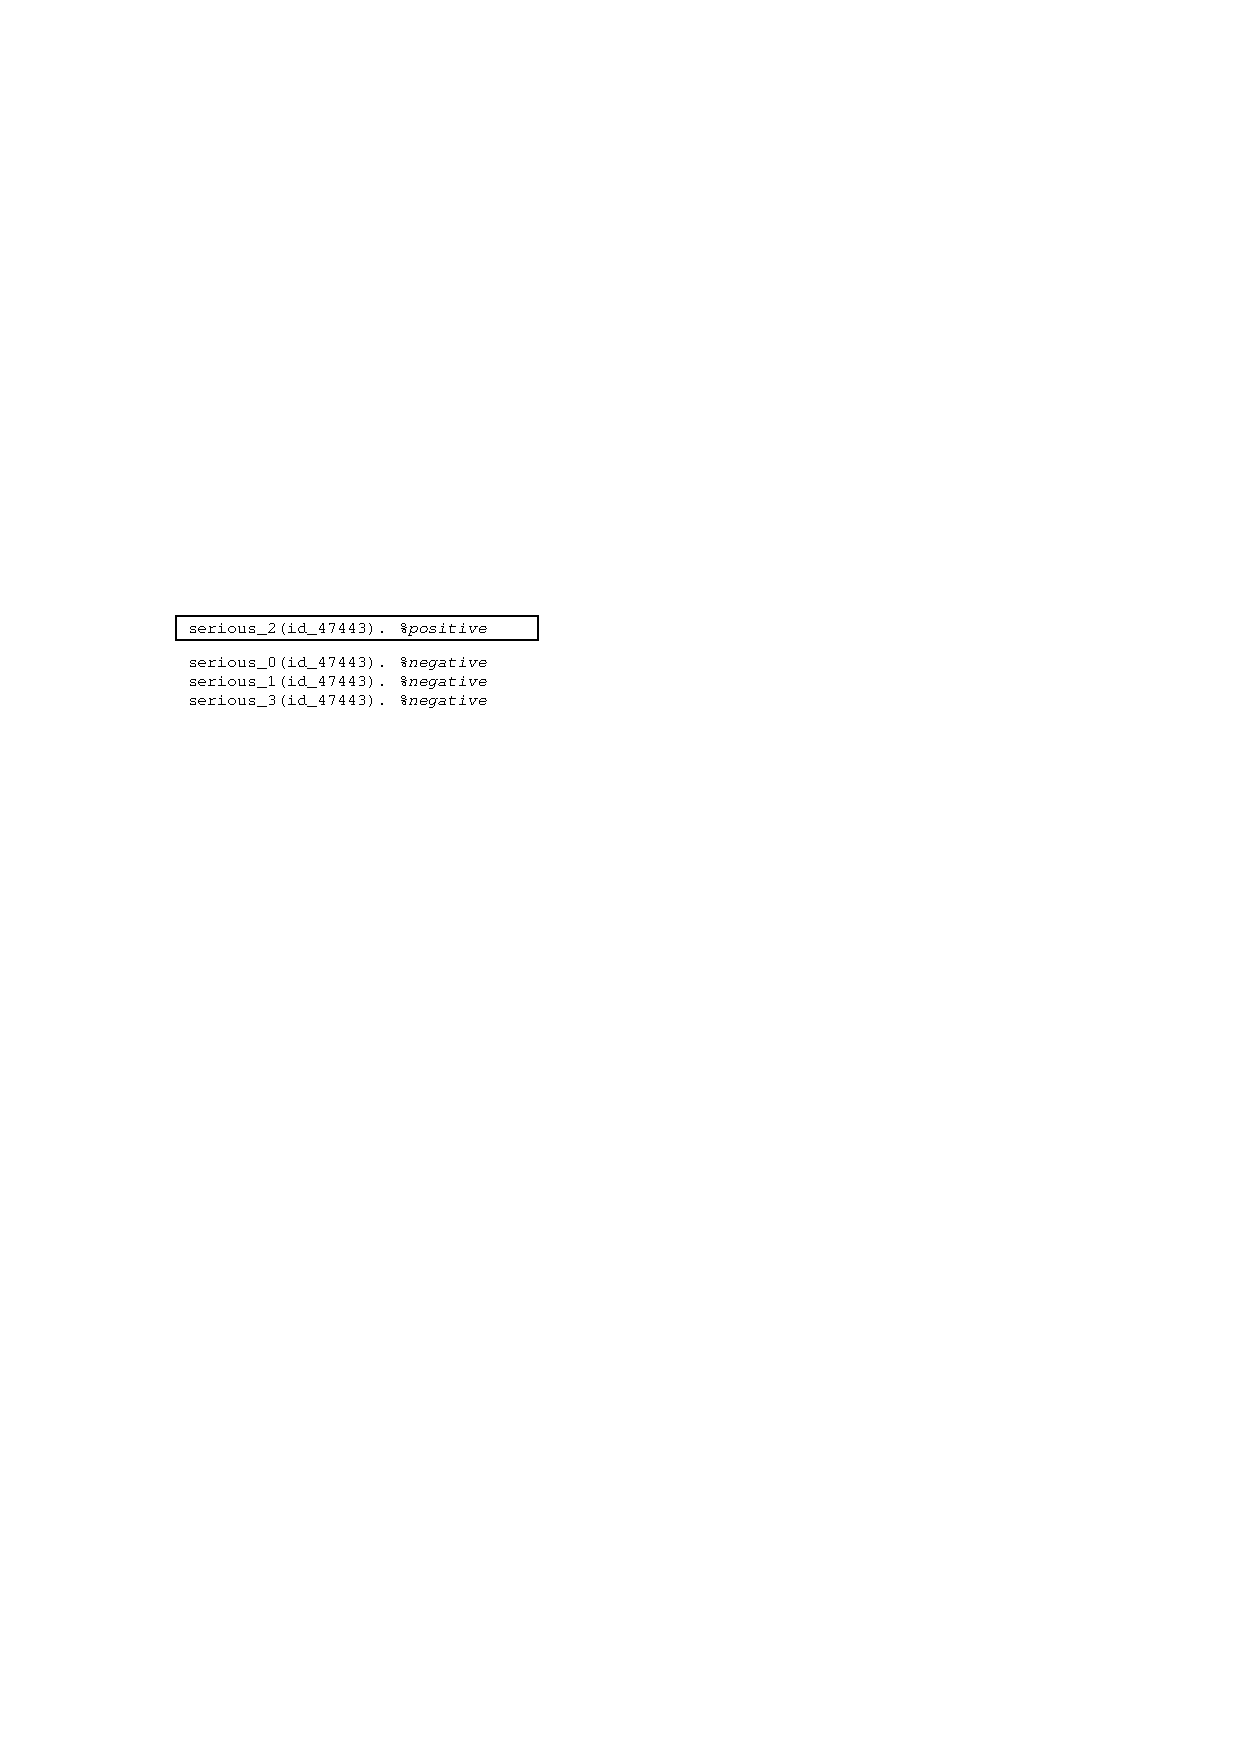
\includegraphics[width=\hsize]{img/examples_nonmonot}}
	Monotonized learning examples\\
	\centerline{
\includegraphics[width=\hsize]{img/examples_monot}}
	\caption{Learning examples.}
	\label{img:examples}
\end{minipage}
\hspace{0.5cm}
\begin{minipage}[b]{0.5\hsize}
	\centerline{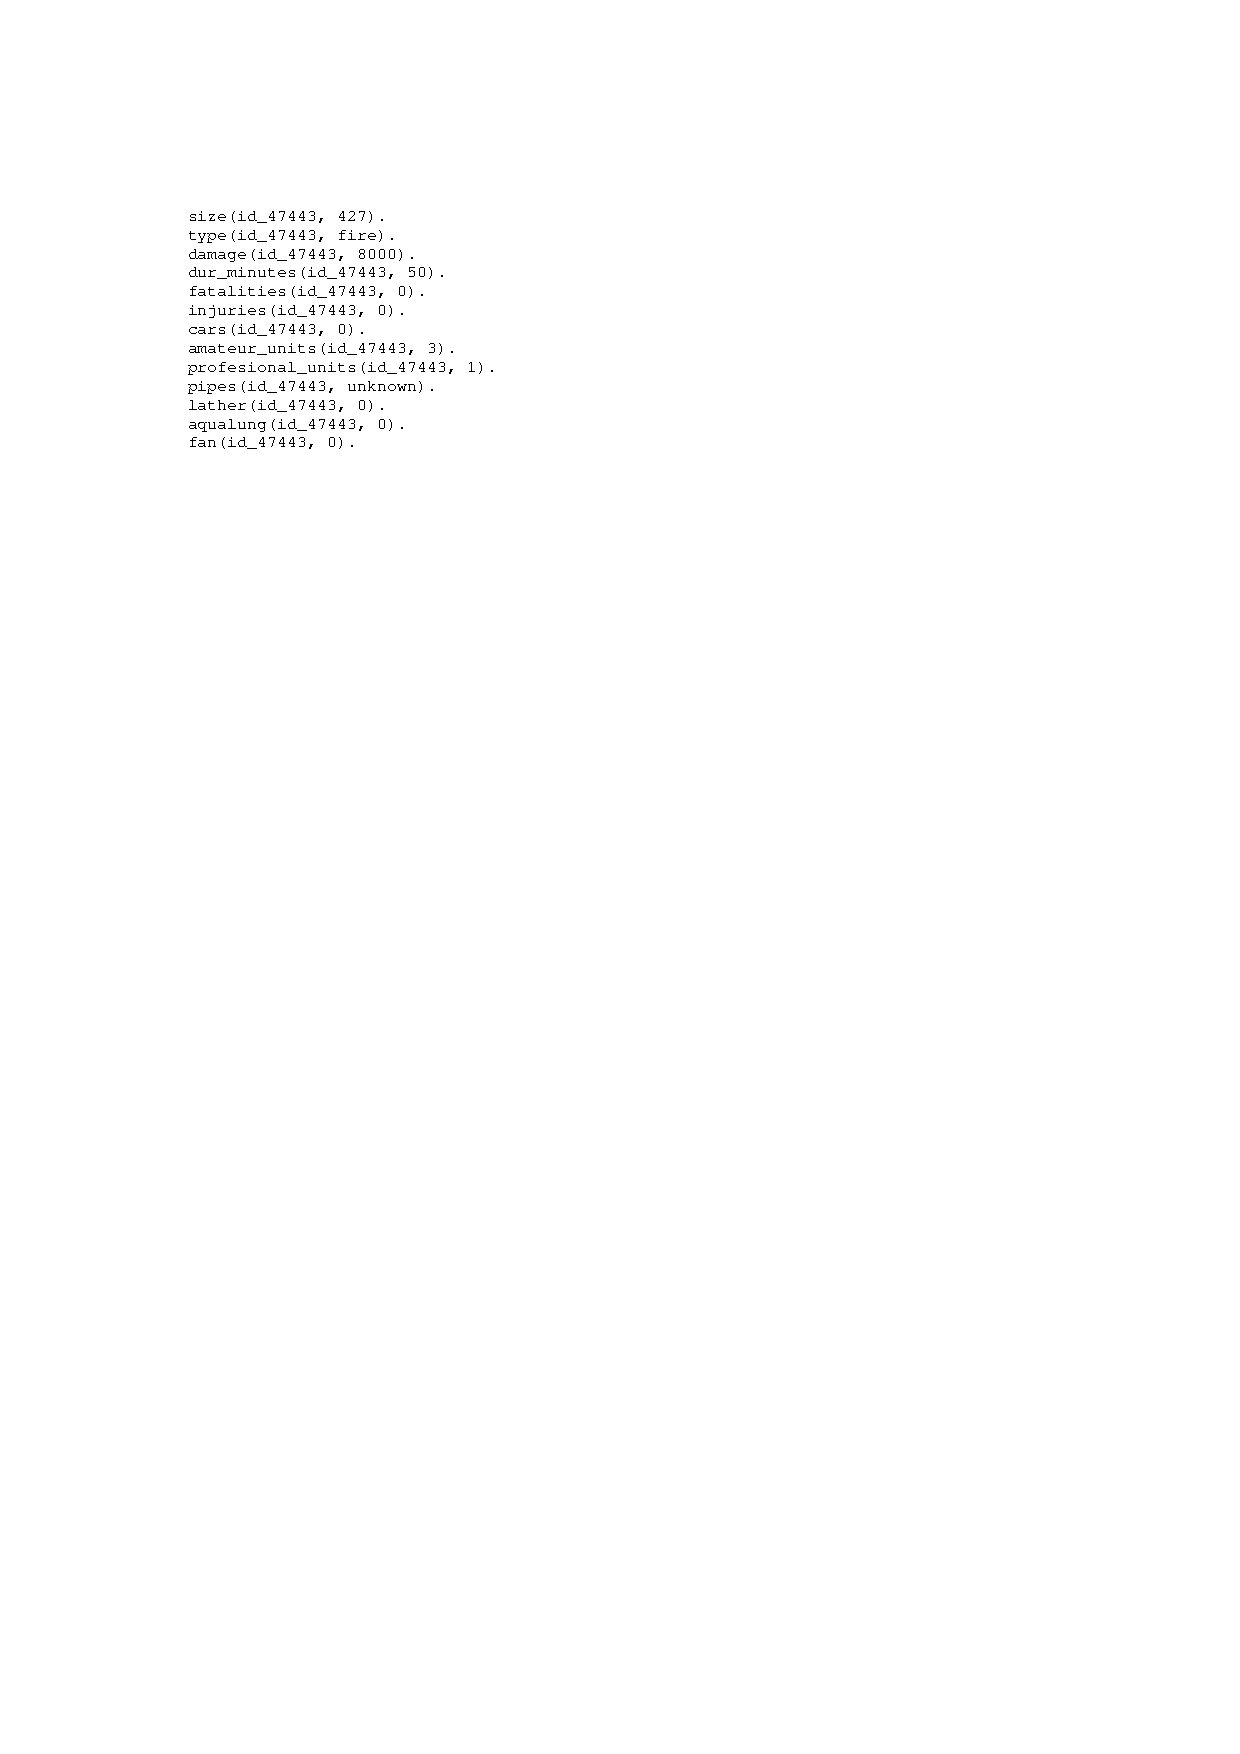
\includegraphics[width=0.835\hsize]{img/crisp_attributes}}
	\caption{$B^{raw}_{T}$ -- crisp attributes.}
	\label{img:crisp_attributes}
\end{minipage}
\end{figure}

\begin{figure}[htb]	
	\centerline{
\includegraphics[width=0.53\hsize]{img/attribute_monotonisation}}
	\caption{Monotonization of attributes (damage\_atl $\leftarrow$ damage)}
	\label{img:attribute_monotonization}
\end{figure}

%
%\begin{figure}[t!]
%Crisp learning examples\\
%\centerline{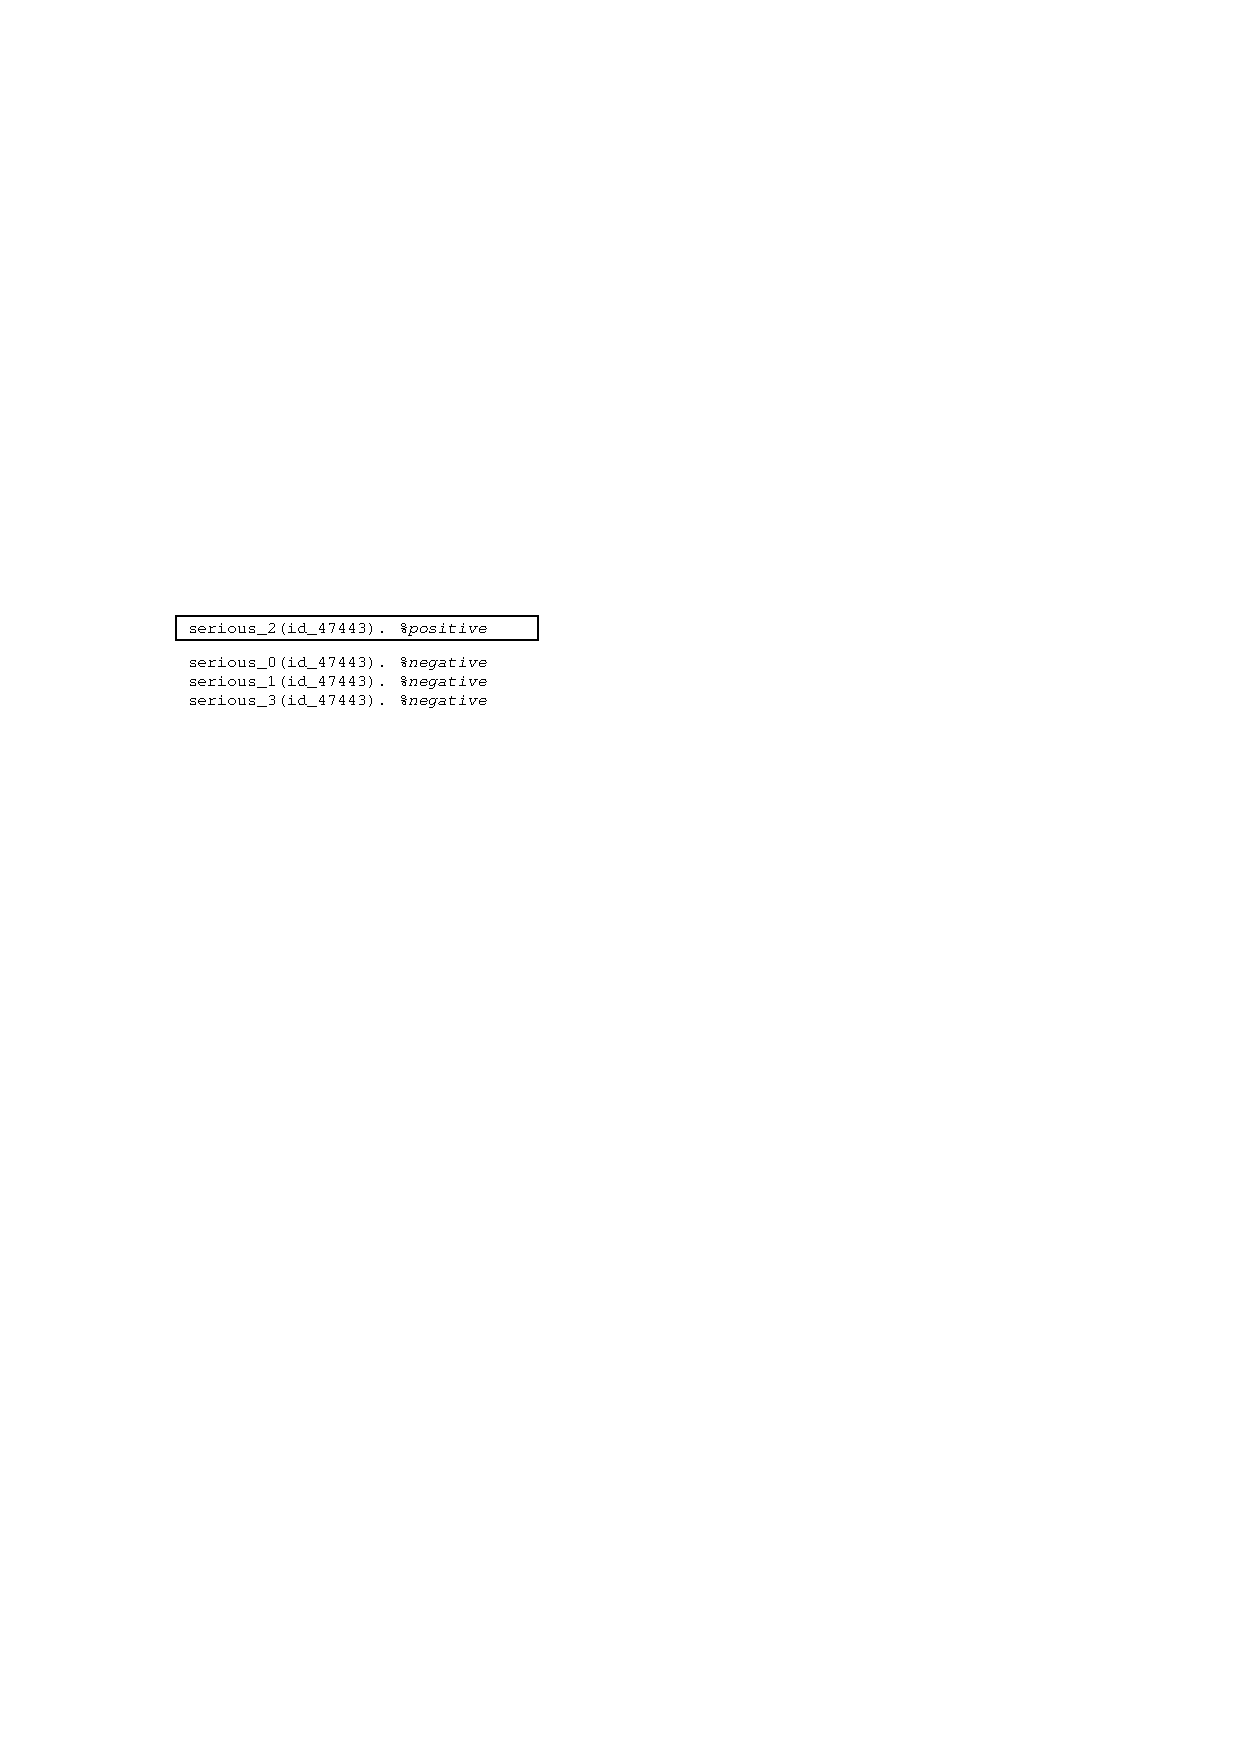
\includegraphics[width=.8\hsize]{img/examples_nonmonot}}
%Monotonized learning examples\\
%\centerline{
\includegraphics[width=.8\hsize]{img/examples_monot}}
%\caption{Learning examples.}
%\label{img:examples}
%\end{figure}
%
%\begin{figure}[t!]
%damage $\rightarrow$ damage\_atl\\
%\centerline{
\includegraphics[width=.8\hsize]{img/attribute_monotonisation}}
%\caption{Monotonization of attributes.}
%\label{img:attribute_monotonization}
%\vspace{-0.5cm}
%\end{figure}



%%%%%%%%%%%%%%%%%%%%%%%%%%%%%%%%%%%%%%%%%%%%%%%%%%%%%%%%%%%%%%%%%%%%%%%%%%%%%%%%%%%%%%%%%%%%%%%%%
\subsection{Data transformation} \label{sec:data_transformation}
%%%%%%%%%%%%%%%%%%%%%%%%%%%%%%%%%%%%%%%%%%%%%%%%%%%%%%%%%%%%%%%%%%%%%%%%%%%%%%%%%%%%%%%%%%%%%%%%%

To use ILP for the classification task we have to translate the input data to the prolog-like logic representation. As already described in previous sections, the transformations for the crisp and for the fuzzy approach are different. Here we will describe the implementation details about the construction of~crisp and fuzzy knowledge bases and example sets.

For the construction of the crisp example set $E_t$ in our application we encode it in the predicate \texttt{serious\_t}, for the construction of the fuzzy (or monotonized) example set $E_{\ge t}$ we encode it in the predicate \texttt{serious\_atl\_t} in our application, see Fig.~\ref{img:examples}.



For the construction of crisp background knowledge $B^{raw}_{T}$ we use a simple translation of the data to the prolog predicates (illustrated on the Fig.~\ref{img:crisp_attributes}). 


%\begin{figure}
%\centerline{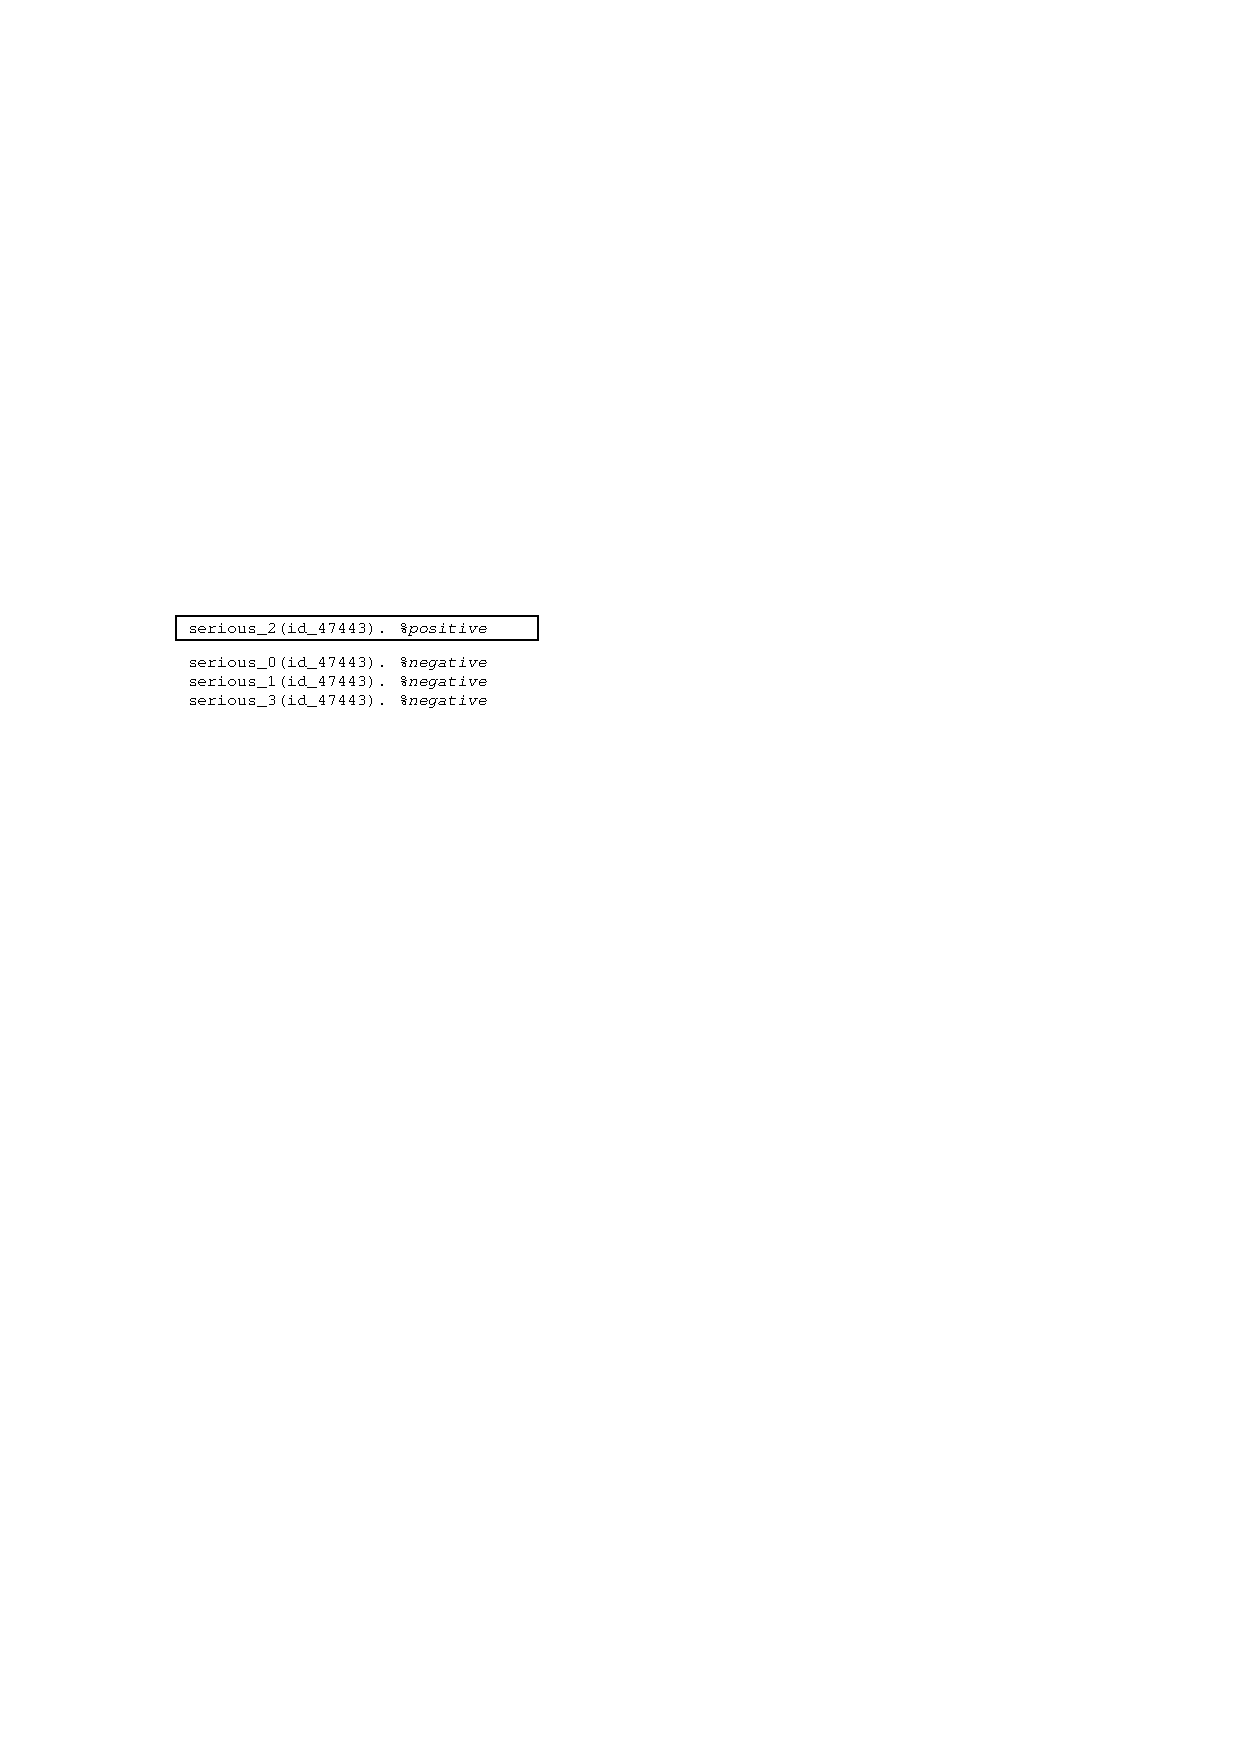
\includegraphics[width=.8\hsize]{img/examples_nonmonot}}
%\caption{Crisp learning examples.}
%\label{img:examples_nonmonot}
%\end{figure}
%
%\begin{figure}
%\centerline{
\includegraphics[width=.9\hsize]{img/examples_monot}}
%\caption{Monotonized learning examples.}
%\label{img:examples_monot}
%\end{figure}
%
For the construction of monotonized background knowledge $B^{mon}_T$ we use rules, here illustrated on predicates \texttt{damage} and \texttt{damage\_atl}, see Fig.~\ref{img:attribute_monotonization}. Here, the first rule deals with \texttt{unknown} values and the second constructs the translation.

Once we have the learning examples and the background knowledge, we can run the ILP inductive learning procedure and obtain learned rules (or a hypothesis). According to the kind of the ILP task (crisp or monotonized) we obtain corresponding kind (crisp or monotonized) of rules (see e.g. Fig.~\ref{img:rules}). But these rules cannot be used to solve the classification task directly. 

Fig.~\ref{img:conversion} hows an example of rules for conversion of the result of a monotonized hypothesis to one crisp seriousness category. Here the negation ``\texttt{not(serious\_atl\_3(ID))}'' means a standard Prolog \emph{negation as failure}. 

\begin{figure}
\centerline{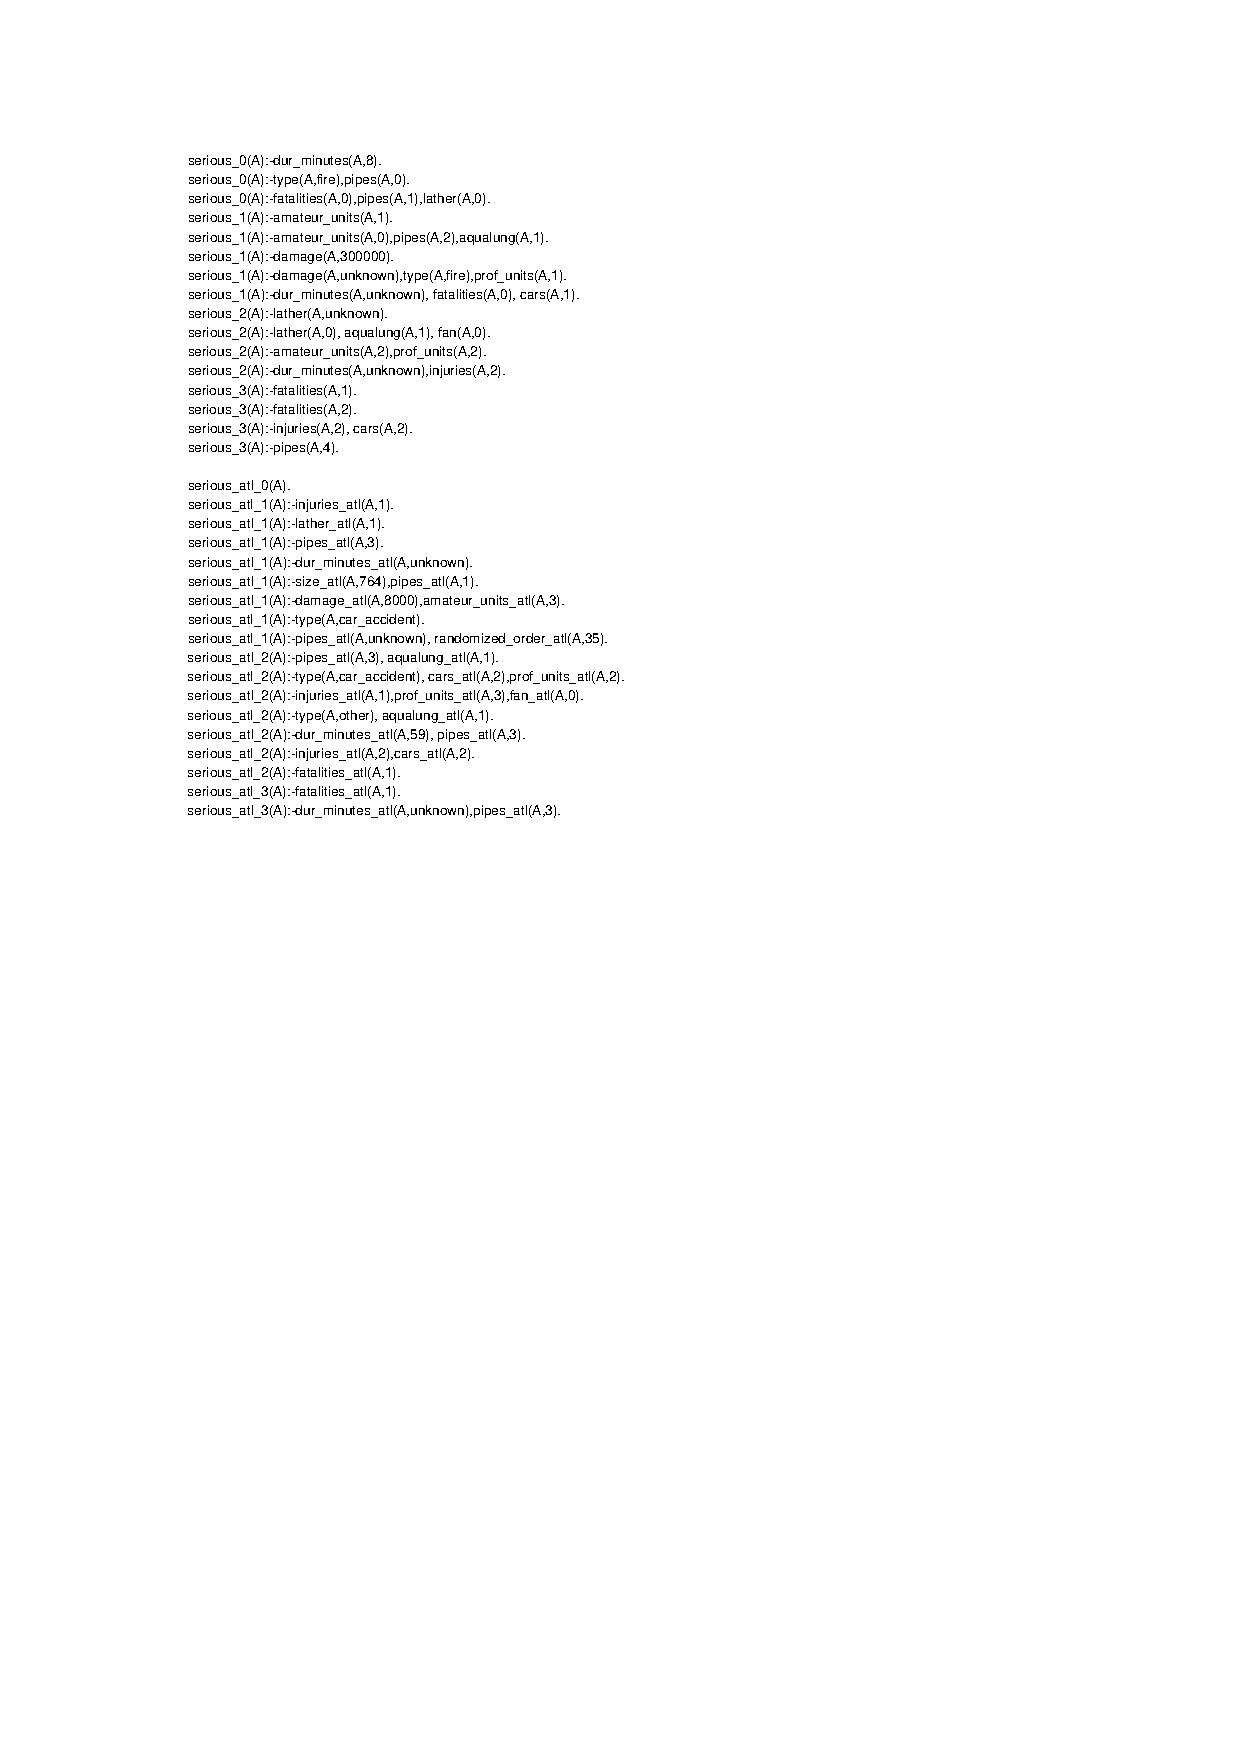
\includegraphics[width=0.6\hsize,height=0.65\hsize]{img/rules}}
\caption{Crisp \& monotonized hypotheses}
\label{img:rules}
\end{figure}

\begin{figure}
\centerline{
\includegraphics[width=0.52\hsize]{img/conversion}}
\caption{Conversion rules for monotonized hypotheses (\texttt{serious\_t} $\leftarrow$ \texttt{serious\_atl\_t})}
\label{img:conversion}
\end{figure}

%\begin{figure}
%\centerline{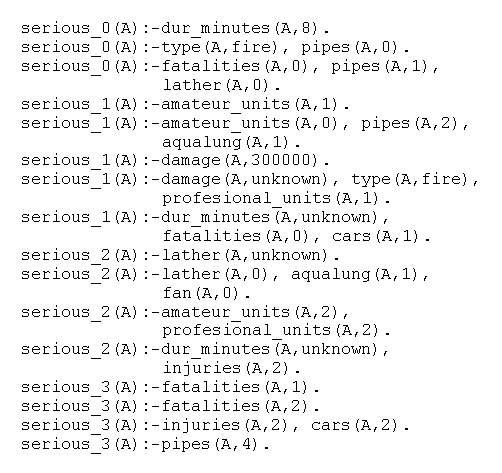
\includegraphics[width=\hsize]{img/rules_nonmonot}}
%\caption{Crisp hypothesis}
%\label{img:rules_nonmonot}
%\end{figure}
%
%\begin{figure}
%\centerline{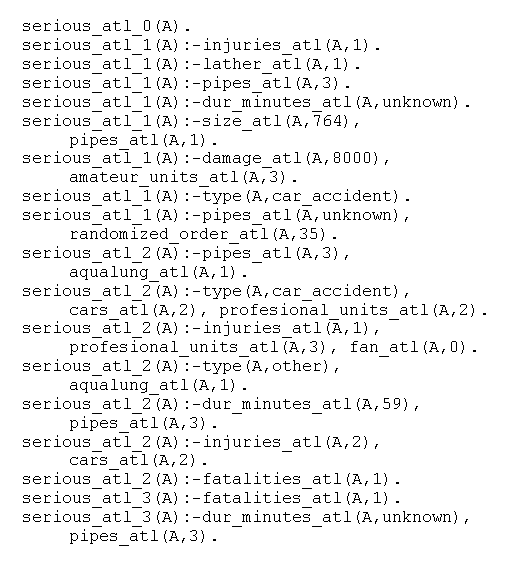
\includegraphics[width=\hsize]{img/rules_monot}}
%\caption{Monotonized hypothesis}
%\label{img:rules_monot}
%\end{figure}


\begin{figure}
\centerline{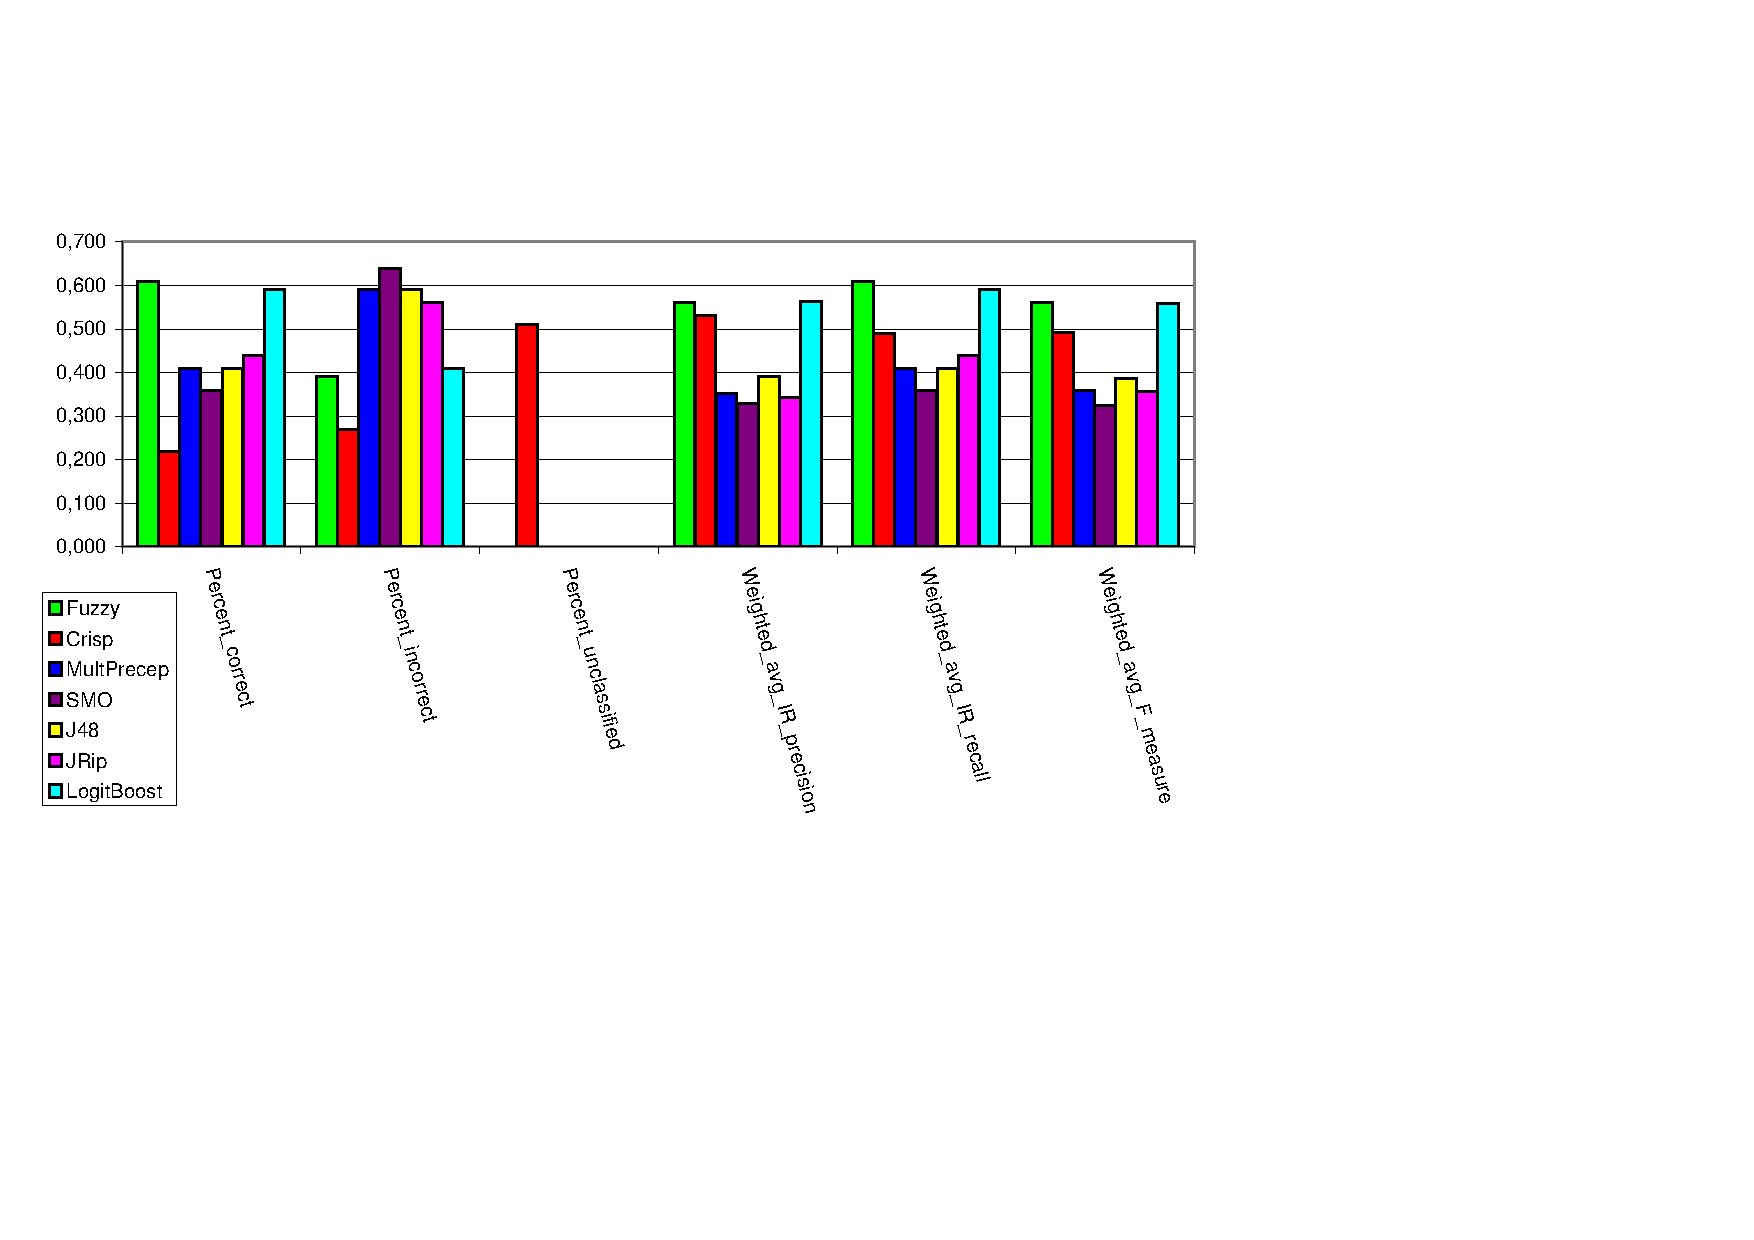
\includegraphics[width=\hsize]{img/2x10cross}}
\caption{Evaluation of the methods -- average values}
\label{img:graph2x10}
\end{figure}


\begin{table}[thb]
\caption{Evaluation of the methods in 2 times 10-fold cross validation}
\label{tab:table2x10}
\scriptsize
{\centering \begin{tabular}{lr@{\hspace{0cm}}c@{\hspace{0cm}}rr@{\hspace{0cm}}c@{\hspace{0cm}}r@{\hspace{0.05cm}}cr@{\hspace{0cm}}c@{\hspace{0cm}}r@{\hspace{0.05cm}}cr@{\hspace{0cm}}c@{\hspace{0cm}}r@{\hspace{0.05cm}}cr@{\hspace{0cm}}c@{\hspace{0cm}}r@{\hspace{0.05cm}}cr@{\hspace{0cm}}c@{\hspace{0cm}}r@{\hspace{0.05cm}}cr@{\hspace{0cm}}c@{\hspace{0cm}}r@{\hspace{0.05cm}}c}
\\
\hline
& \multicolumn{3}{c}{Fuzzy}& \multicolumn{4}{c}{Crisp} & \multicolumn{4}{c}{MultPerc} & \multicolumn{4}{c}{SMO} & \multicolumn{4}{c}{J48} & \multicolumn{4}{c}{JRip} & \multicolumn{4}{c}{LBoost} \\
\hline
Corr	& 0.61 & $\pm$ & .19 & .22 & $\pm$ & .17 & $\bullet$ & .41 & $\pm$ & .19 & $\bullet$ & .36 & $\pm$ & .24 & $\bullet$ & .41 & $\pm$ & .22 & $\bullet$ & .44 & $\pm$ & .17 & $\bullet$ & .59 & $\pm$ & .26 &        \\
Incor	& .39 & $\pm$ & .19 & .27 & $\pm$ & .24 &         	& .59 & $\pm$ & .19 & $\circ$ 	& .64 & $\pm$ & .24 & $\circ$ 	& .59 & $\pm$ & .22 & $\circ$ 	& .56 & $\pm$ & .17 & $\circ$ 	& .41 & $\pm$ & .26 &        \\
Uncl	& .00	& $\pm$ & .00	& .51 & $\pm$ & .29 & $\circ$ 	& .00 & $\pm$ & .00 &         	& .00 & $\pm$ & .00 &         	& .00 & $\pm$ & .00 &         	& .00 & $\pm$ & .00 &         	& .00 & $\pm$ & .00 &        \\
Prec	& .56 & $\pm$ & .24 & .53 & $\pm$ & .37 &         	& .35 & $\pm$ & .20 & $\bullet$ & .33 & $\pm$ & .26 &         	& .39 & $\pm$ & .22 &         	& .34 & $\pm$ & .21 & $\bullet$ & .56 & $\pm$ & .28 &        \\
Rec		& .61 & $\pm$ & .19 & .49 & $\pm$ & .32 &         	& .41 & $\pm$ & .19 & $\bullet$ & .36 & $\pm$ & .24 & $\bullet$ & .41 & $\pm$ & .22 & $\bullet$ & .44 & $\pm$ & .17 & $\bullet$ & .59 & $\pm$ & .26 &        \\
F			& .56 & $\pm$ & .20 & .49 & $\pm$ & .33 &         	& .36 & $\pm$ & .19 & $\bullet$ & .32 & $\pm$ & .24 & $\bullet$ & .39 & $\pm$ & .21 &         	& .36 & $\pm$ & .19 & $\bullet$ & .56 & $\pm$ & .27 &        \\
\hline
\multicolumn{21}{c}{$\circ$, $\bullet$ statistically significant improvement or degradation}\\
\end{tabular} \scriptsize \par}
\scriptsize
\smallskip
Legend:\\
{\centering
\begin{tabular}{p{2cm}@{}p{10.5cm}}\\
Fuzzy \dotfill{}& czsem.ILP.FuzzyILPClassifier '' \\
Crisp \dotfill{} & czsem.ILP.CrispILPClassifier '' \\
MultPerc \dotfill{} & functions.MultilayerPerceptron '-L 0.3 -M 0.2 -N 500 -V 0 -S 0 -E 20 -H a' \\
SMO \dotfill{} & functions.SMO '-C 1.0 -L 0.0010 -P 1.0E-12 -N 0 -V -1 -W 1 -K \textbackslash"functions.supportVector.PolyKernel -C 250007 -E 1.0\textbackslash"' \\
J48 \dotfill{} & trees.J48 '-C 0.25 -M 2' \\
JRip \dotfill{} & rules.JRip '-F 3 -N 2.0 -O 2 -S 1' \\
LBoost \dotfill{} & meta.LogitBoost '-P 100 -F 0 -R 1 -L -1.7976931348623157E308 -H 0.1 -S 1 -I 10 -W trees.DecisionStump' \\
\\
Corr \dotfill{} & Percent correct\\
Inor \dotfill{} & Percent incorrect\\
Uncl \dotfill{} & Percent unclassified\\
Prec \dotfill{} & Weighted avg IR precision\\
Rec \dotfill{} 	& Weighted avg IR recall\\
F \dotfill{} 		& Weighted avg F measure\\
\end{tabular}
}
\end{table}

%%%%%%%%%%%%%%%%%%%%%%%%%%%%%%%%%%%%%%%%%%%%%%%%%%%%%%%%%%%%%%%%%%%%%%%%%%%%%%%%%%%%%%%%%%%%%%%%%
\section{Results} \label{sec:results}
%%%%%%%%%%%%%%%%%%%%%%%%%%%%%%%%%%%%%%%%%%%%%%%%%%%%%%%%%%%%%%%%%%%%%%%%%%%%%%%%%%%%%%%%%%%%%%%%%

The Fig.~\ref{img:rules} summarizes sets of obtained rules from two experiments: 
\begin{enumerate}
	\item experiments with $E_t$ and $B^{raw}_{T}$ 
	\item experiments with $E_{\ge t}, {B}^{mon}_T$.
\end{enumerate}
In both experiments learning and testing examples and the background knowledge had their origin in the same data (the same accidents) but they differ in the form of the ILP task (crisp and monotonized).

We have evaluated these two methods and compared them with other learning tools used in data mining. To make the comparison clear and easy to perform, we have implemented an interface between the ILP methods and the Weka data mining software\footnote{\url{http://www.cs.waikato.ac.nz/ml/weka/}}. The interface makes it possible to use the ILP methods as an ordinary Weka classifier for any\footnote{For the fuzzy ILP method, there is a requirement on the target (class) attribute: it has to be monotonizable (e.g. numeric).} classification task inside the Weka software. We used the Weka Experimenter and performed experiments with additional classifiers:
%Jmenovit� rozhodovac� stromy J48 \cite{biblio:J48}, Support vector machine klasifik�tor SMO \cite{biblio:SMO} a v�cevrstv� perceptron \cite{biblio:bishop-1995}.
\begin{itemize}
	\item Multilayer Perceptron \citep{biblio:bishop-1995},
	\item Support Vector Machine classifier SMO \citep{biblio:SMO},
	\item J48 decision tree \citep{biblio:J48},
	\item JRip rules \citep{weka:JRip} and
	\item Additive logistic regression LogitBoost \citep{biblio:LogitBoost},
\end{itemize}
and evaluated all the methods two times by 10-fold cross validation on our data (section~\ref{sec:experiment_desc}). The obtained results (average values) are described by the graph in the Fig.~\ref{img:graph2x10} and in the Table~\ref{tab:table2x10} (with standard deviations and decorated statistically significant values).




%%%%%%%%%%%%%%%%%%%%%%%%%%%%%%%%%%%%%%%%%%%%%%%%%%%%%%%%%%%%%%%%%%%%%%%%%%%%%%%%%%%%%%%%%%%%%%%%%
\section{Results2 - stary clanek} \label{sec:results2}
%%%%%%%%%%%%%%%%%%%%%%%%%%%%%%%%%%%%%%%%%%%%%%%%%%%%%%%%%%%%%%%%%%%%%%%%%%%%%%%%%%%%%%%%%%%%%%%%%


The Fig.~\ref{img:evaluation} shows the success of these rules on the test data (not used during learning). We have used standard performance measures\footnote{\url{http://en.wikipedia.org/wiki/Precision_and_recall}} often used in information retrieval. There are also exact numbers of \emph{true positives} TP and \emph{false positives} FP from which the performance measures were computed (with respect to the numbers of all testing examples\footnote{These numbers are written in the Fig.~\ref{img:evaluation} in small frames under each test set label.}).

Naturally monotonized hypotheses $H_{\ge t}$ were tested on monotonized examples $E_{\ge t}$ (double-line frame in the Fig.~\ref{img:rules}) and similarly for the crisp case $H_t, E_t$ (dashed-line frame in the Fig.~\ref{img:rules}).
%Experiments with $E_t$ and $B^{raw}_{T}$ %Results of experiments with $E_t$ and $B^{raw}_{T}$ 
%gave following rule set, see Fig.~\ref{img:rules_nonmonot}.
%Evaluation of learning is depicted in the Fig.~\ref{img:evaluation}.
%\subsection{Experiments $E_{\ge t}, {B}^{mon}_T$}
%Evaluation of learning is depicted in the green area of Fig.~\ref{img:evaluation}.
%\subsection{Evaluation and comparison }

We wanted to compare raw and monotonized learning tasks. As they run on different example sets we had to translate results of one learning (rules with head \texttt{serious\_t}) to results of second learning (rules with head \texttt{serious\_atl\_t}). Logic programming translation rules are depicted on the Fig.~\ref{img:monot2nomon_and_invert}. Here the negation ``\texttt{not(serious\_atl\_3(ID))}'' means a standard Prolog \emph{negation as failure}. 

Then the comparison of both learnings is possible, see the numbers in white areas of Fig.~\ref{img:evaluation}.


\begin{figure}[ht]
\begin{minipage}[b]{0.5\hsize}
	\centering
		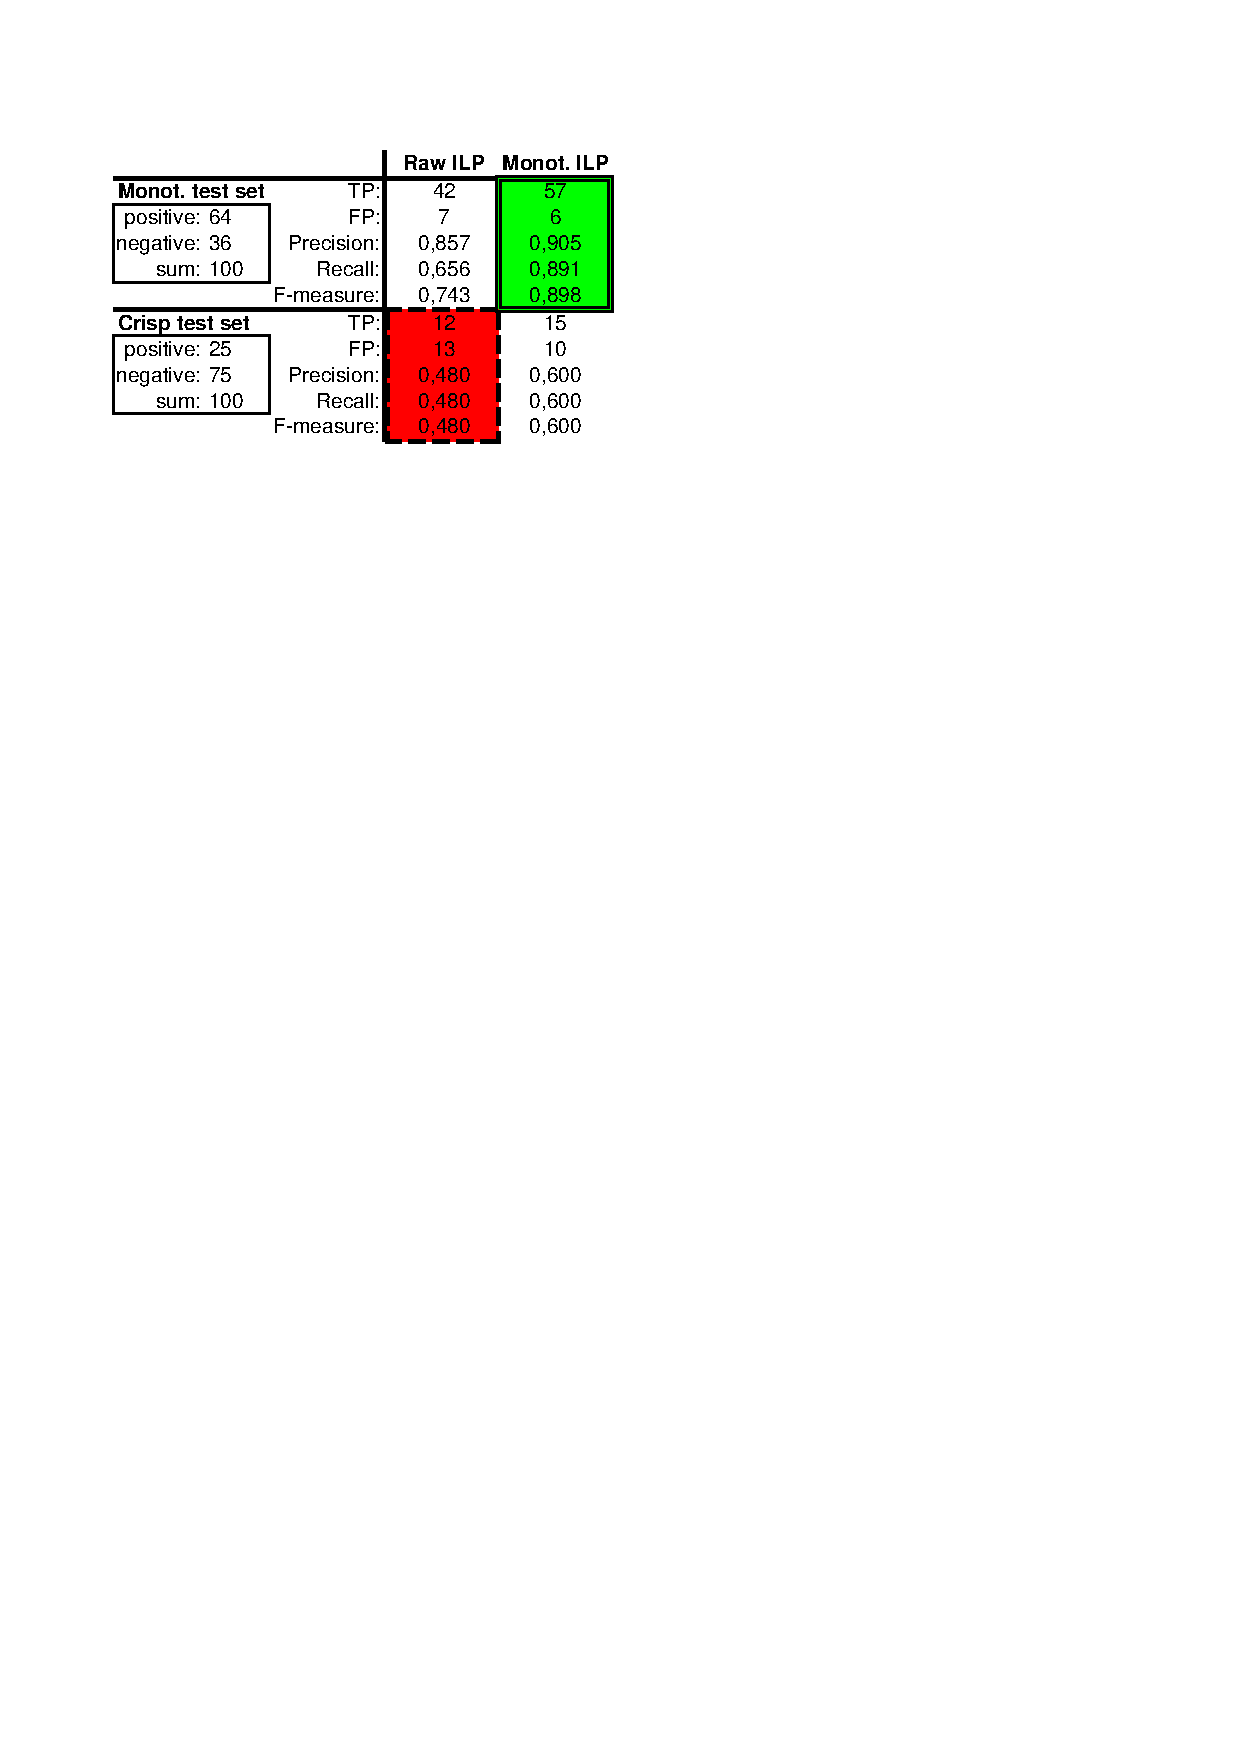
\includegraphics[width=\hsize]{img/Evaluation}
\caption{Evaluation results}
\label{img:evaluation}
\end{minipage}
\hspace{0.5cm}
\begin{minipage}[b]{0.5\hsize}
crisp $\rightarrow$ monotone\\
	{\centering
		
\includegraphics[width=\hsize]{img/nomon2monot}}
monotone $\rightarrow$ crisp\\
	{\centering
		\\
\includegraphics[width=\hsize]{img/monot2nomon}}
\caption{Conversion of results}
\label{img:monot2nomon_and_invert}
\end{minipage}
\end{figure}


%\begin{figure}
%\centerline{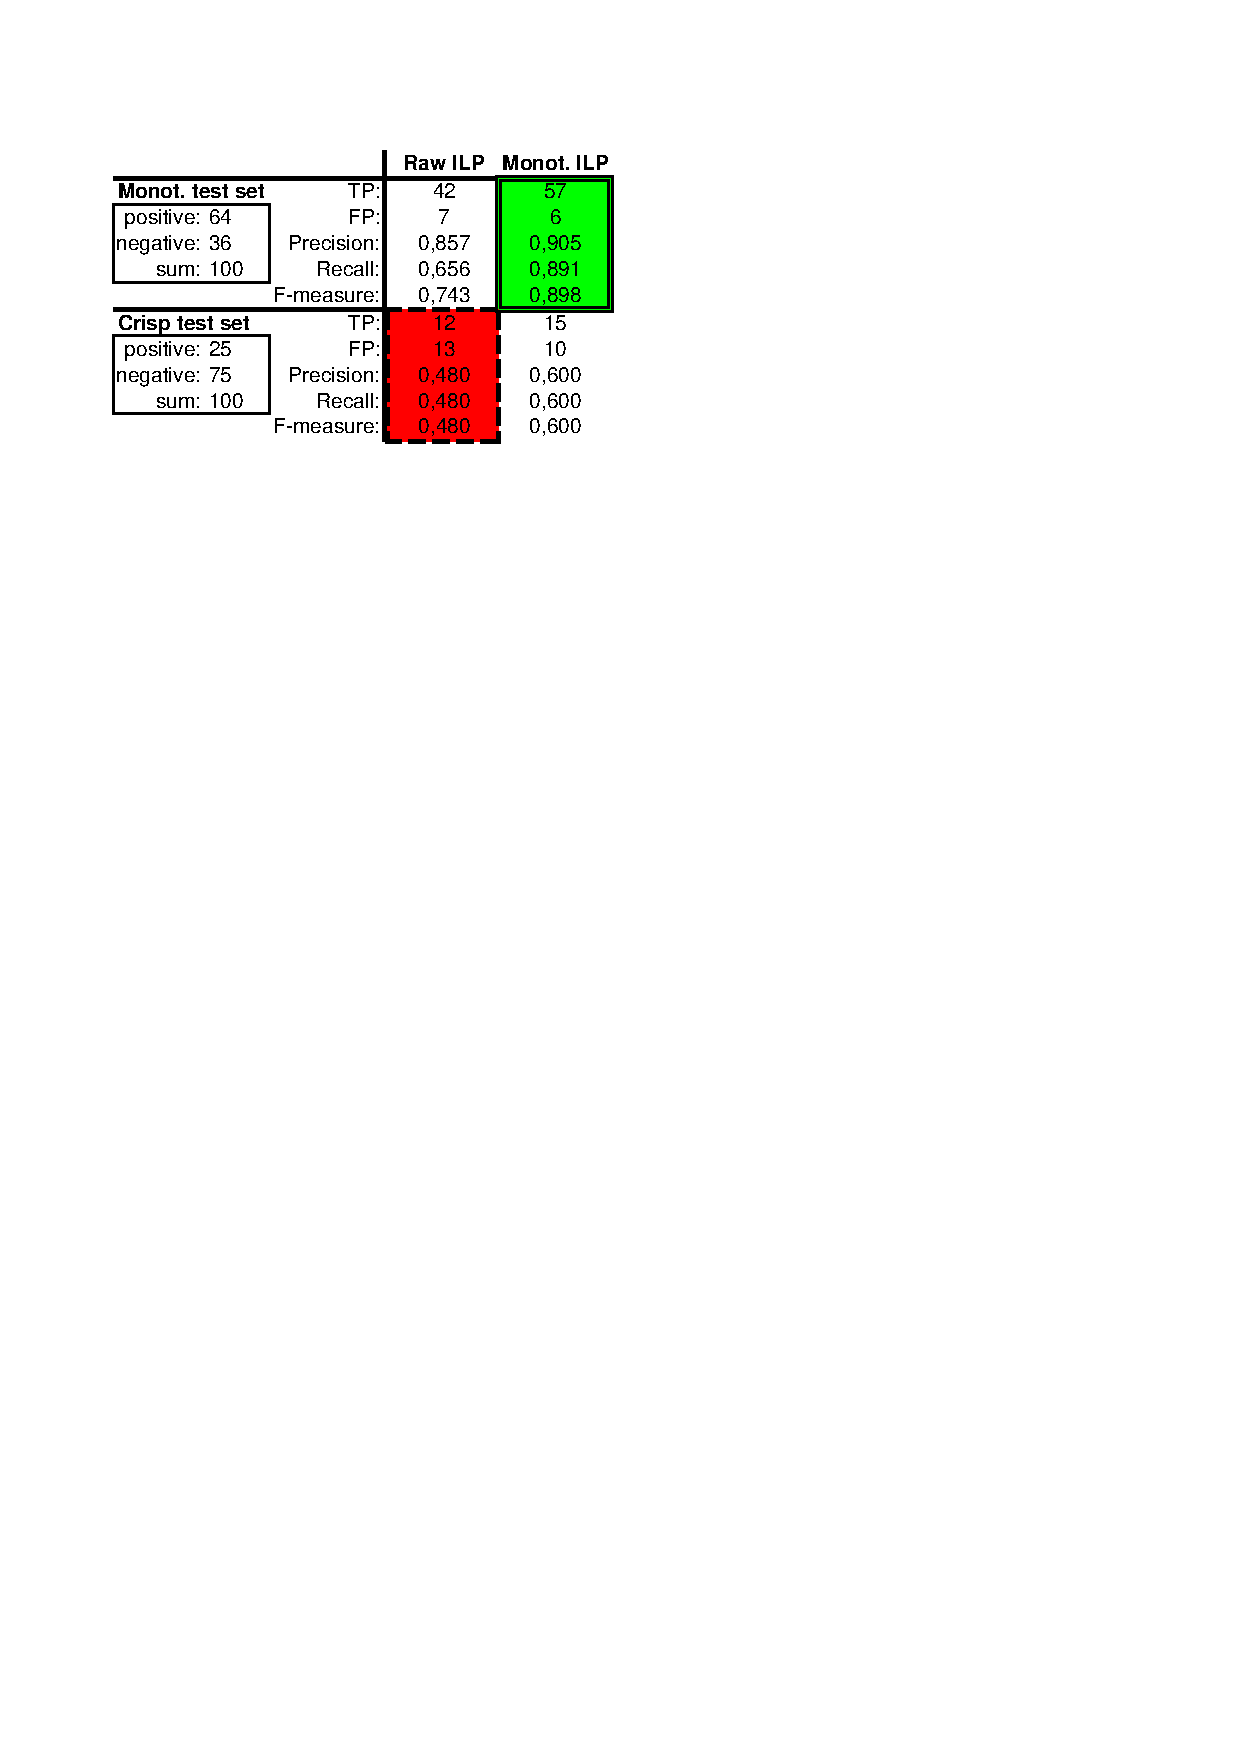
\includegraphics[width=0.8\hsize]{img/Evaluation}}
%\caption{Evaluation results}
%\label{img:evaluation}
%\end{figure}
%
%
%\begin{figure}
%crisp $\rightarrow$ monotone\\
%\centerline{
\includegraphics[width=.8\hsize]{img/nomon2monot}}
%
%monotone $\rightarrow$ crisp\\
%\centerline{
\includegraphics[width=.8\hsize]{img/monot2nomon}}
%\caption{Conversion of results}
%\label{img:monot2nomon_and_invert}
%\end{figure}

%\begin{figure}
%\centerline{
\includegraphics[width=.8\hsize]{img/nomon2monot}}
%\caption{Results conv.: crisp $\rightarrow$ monotone.}
%\label{img:nomon2monot}
%\end{figure}
%
%
%
%
%\begin{figure}
%\centerline{
\includegraphics[width=.8\hsize]{img/monot2nomon}}
%\caption{Results conv.: monotone $\rightarrow$ crisp.}
%\label{img:monot2nomon}
%\end{figure}


%%%%%%%%%%%%%%%%%%%%%%%%%%%%%%%%%%%%%%%%%%%%%%%%%%%%%%%%%%%%%%%%%%%%%%%%%%%%%%%%%%%%%%%%%%%%%%%%%
\section{Conclusion}
%%%%%%%%%%%%%%%%%%%%%%%%%%%%%%%%%%%%%%%%%%%%%%%%%%%%%%%%%%%%%%%%%%%%%%%%%%%%%%%%%%%%%%%%%%%%%%%%%
In this paper we have presented a fuzzy system which provides a fuzzy classification of textual web reports. Our approach was based on usage of third party linguistic analyzers, our previous work on web information extraction and fuzzy inductive logic programming.

Main contributions are formal models and prototype implementation of the system and evaluation experiments with the Fuzzy ILP classification method.

Experiments have shown better results of fuzzy approach. We see the difference in the fact that monotonization leads to the extension of the learning domain.

%Use of ILP was necessary for multirelational character of extracted data (relational representation of XML like form of PDT2.0 tectogramatical trees). 
%
%System need user assistance: of a skilled user in annotating data for extraction and an unskilled user for classification of a small training example set. This feature is especially important, because in Internet application, we cannot expect an unskilled user to classify a big number of examples 

\section*{Acknowledgments}
This work was partially supported by Czech projects: GACR P202/10/0761, GACR-201/09/H057, GAUK 31009 and MSM-0021620838.

\section*{References}

\bibliographystyle{elsarticle-harv}
\bibliography{DedVojVom_SAIAW_FuzzyILP}





\end{document}



%%% Local Variables: 
%%% mode: latex
%%% TeX-master: t
%%% End: 
